\newif\ifglobal

%%%%%%%%%%%%%%%%%%%%%%%
%%% Compile to view %%%
%%%%%%%%%%%%%%%%%%%%%%%

%%%%%%%%%%%%%%%%%%%%%%%%%%%%%%%%%%%%%%%%%%%%%%%%%%%
%%% Readme:                                     %%%
%%% https://www.overleaf.com/read/bwdjvfjksvjy/ %%%
%%%%%%%%%%%%%%%%%%%%%%%%%%%%%%%%%%%%%%%%%%%%%%%%%%%

% >>> M?: marks a module setting number or important notice

% >>> M4: Set {./relative-path} to external files for this module <<<
\def \modulefiles {./03-I2S}
% To add an external file, use:
% (Replace '---' with actual filename)
% '\input{\modulefiles/tables/---.tex}' for tables
% '\includegraphics{\modulefiles/figures/---}' for figures
% '\subfile{\modulefiles/---}' for register files

% >>> M1: This module is in global project? <<<
% 'YES' - uncomment; 'NO' - comment out
\globaltrue

\ifglobal
    \documentclass[main\_\_CN.tex]{subfiles}

\else
    % Font "FandolSong-Regular" used by ctex does not have GSUB table.
    % It causes warnings that do not affect compilation and can be ignored.
    \PassOptionsToPackage{quiet}{fontspec}

    \documentclass[openany, 10pt]{book}

    % >>> M2: In ./00-shared/preamble-trm-module, also find
    %         settings for visibility of todo notes, watermark <<<
    \usepackage{preamble-trm-module}


    % Enable Chinese typesetting
    \usepackage{ctex}

    % >>> M3: Temporary labels in Chinese
    %         you can add your own labels there <<<
    \myexternaldocument{./00-shared/temp-labels-cn}

\fi %\ifglobal


\setcounter{secnumdepth}{4}

% >>> M4: Set {./relative-path} to external files for this module <<<
% \def \modulefiles {./03-I2S}
% To add an external file, use:
% (Replace '---' with actual filename)
% '\input{\modulefiles/tables/---.tex}' for tables
% '\includegraphics{\modulefiles/figures/---}' for figures
% '\subfile{\modulefiles/---}' for register files


% >>> M5: If this module needs any updates in
% './00-shared/preamble-trm-module.sty'
% (include additional package, etc.), contact your module PM
% or create the file './00-shared/changelog.tex' make the
% necessary updates yourself and document them in this file <<<


\begin{document}


% Sets language into which pre-defined bits of text are translated
\selectlanguage{chinese}

% Do not delete this block
\ifglobal
% Add the following front matter if
% this module is outside of global project
\else
    \InputIfFileExists{readme}{}{}
    {\let\clearpage\relax \listoftodos}
    \tableofcontents
    %\listoftables
    %\listoffigures
\fi


%%%%%%%%%%%%%%%%%%%%%%%%%
%%% TRM Module Begins %%%
%%%%%%%%%%%%%%%%%%%%%%%%%
%%%%%%%%%%%%%%%%%%%%%%%%%
%%% 重要!!! %%%
% 本章节是从 ESP32-C3 I2S 直接复制过来的。请基于这个版本进行修改
%%%%%%%%%%%%%%%%%%%%%%%%%

\hypertarget{i2s}{}
\chapter{I2S 控制器 (I2S)}
\label{mod:i2s}

\section{概述}
\chipname{} 内置两个 I2S 接口(即 I2S\regindex{0} 和 I2S\regindex{1}),为多媒体应用,尤其是为数字音频应用提供了灵活的数据通信接口。


I2S 标准总线定义了三种信号:串行时钟信号 BCK、字选择信号 WS 和串行数据信号 SD。一个基本的 I2S 数据总线有一个主机和一个从机。主机和从机的角色在通信过程中保持不变。\chipname{} 的 I2S 模块包含独立的发送单元和接收单元,能够保证优良的通信性能。

\begin{tiplisting}
本章节提供的信息适用于 I2S\regindex{0} 和 I2S\regindex{1}。除非另有说明,本章节中 I2S 及 I2S\regindex{n} 均指代 I2S\regindex{0} 和 I2S\regindex{1}。
\end{tiplisting}

\section{术语}

为了更好地说明 I2S\regindex{n} 的功能,本章使用了以下术语。

\begin{longtable}[c]{ R{4cm} p{10cm} }

\textbf{主机模式}     & I2S\regindex{n} 作为主机,BCK/WS 向外部输出,向从机发送或从其接收数据。 \\
\textbf{从机模式}      & I2S\regindex{n} 作为从机,BCK/WS 从外部输入,从主机接收或向其发送数据。 \\
\textbf{全双工} & 主机与从机之间的发送线和接收线各自独立,发送数据和接收数据同时进行。\\
\textbf{半双工} & 主机和从机只能有一方先发送数据,另一方接收数据。发送数据和接收数据不能同时进行。 \\
\textbf{TDM RX 模式} & 利用时分复用方式接收脉冲编码调制 (PCM) 数据,并将其通过 DMA 存入储存器的模式。信号线包括 BCK、WS 和 DATA。可以接收最多 16 个通道的数据。通过用户配置,可支持 TDM Philips 格式、TDM MSB 对齐格式、TDM PCM 格式等。\\
\textbf{PDM RX 模式} & 接收脉冲密度调制 (PDM) 数据,并将其通过 DMA 存入储存器的模式。信号线包括 WS 和 DATA。通过用户配置,可支持 PDM 标准格式等。\\
\textbf{TDM TX 模式} & 通过 DMA 从储存器中取得脉冲编码调制 (PCM) 数据,并利用时分复用方式将其发送的模式。信号线包括 BCK、WS 和 DATA,可以发送最多 16 个通道的数据。通过用户配置,可支持 TDM Philips 格式、TDM MSB 对齐格式、TDM PCM 格式等。\\
\textbf{PDM TX 模式} & 通过 DMA 从储存器中取得脉冲密度调制 (PDM) 数据,并将其发送的模式。信号线包括 WS 和 DATA。通过用户配置,可支持 PDM 标准格式等。\\
\textbf{PCM-to-PDM TX 模式(仅对 I2S\regindex{0} 有效)} & 通过 DMA 从储存器中取得脉冲编码调制 (PCM) 数据,将其转换为脉冲密度调制 (PDM) 数据,并将其发送的\textbf{主机}模式。信号线包括 WS 和 DATA。通过用户配置,可支持 PDM 标准格式等。\\
\textbf{PDM-to-PCM RX 模式(仅对 I2S\regindex{0} 有效)} & 接收脉冲密度调制 (PDM) 数据,将其转换为脉冲编码调制 (PCM) 数据,并将其通过 DMA 存入储存器的\textbf{主机}模式或\textbf{从机}模式。信号线包括 WS 和 DATA。通过用户配置,可支持 PDM 标准格式等。\\
\end{longtable}


\section{特性}

I2S\regindex{n} 具有以下特性:
\begin{itemize}
    \item 支持主机模式和从机模式
    \item 支持全双工和半双工通信
    \item TX 模块和 RX 模块相互独立
    \item TX 模块和 RX 模块可独立工作或同时工作
    \item 支持多种音频标准:
    \begin{itemize}
        \item TDM Philips 标准
        \item TDM MSB 对齐标准
        \item TDM PCM 标准
        \item PDM 标准
    \end{itemize}
    \item 支持多种 TX/RX 模式
        \begin{itemize}
        \item TDM TX 模式
        \item TDM RX 模式
        \item PDM TX 模式
        \item PDM RX 模式
        \item PCM-to-PDM TX 模式(仅对 I2S\regindex{0} 有效)
        \item PDM-to-PCM RX 模式(仅对 I2S\regindex{0} 有效)
    \end{itemize}
    \item 高精度采样时钟可配置
    \item 支持如下采样频率:8 kHz、16 kHz、32 kHz、44.1 kHz、48 kHz、88.2 kHz、96 kHz、128 kHz 和 192 kHz。注意:不支持从机 192 kHz 32 位模式。
    \item 支持 8/16/24/32 位数据通信
    \item 支持 DMA
    \item 支持 I2S 接口中断
\end{itemize}
\section{系统架构}
\begin{figure}[H]
    \centering
    \fbox{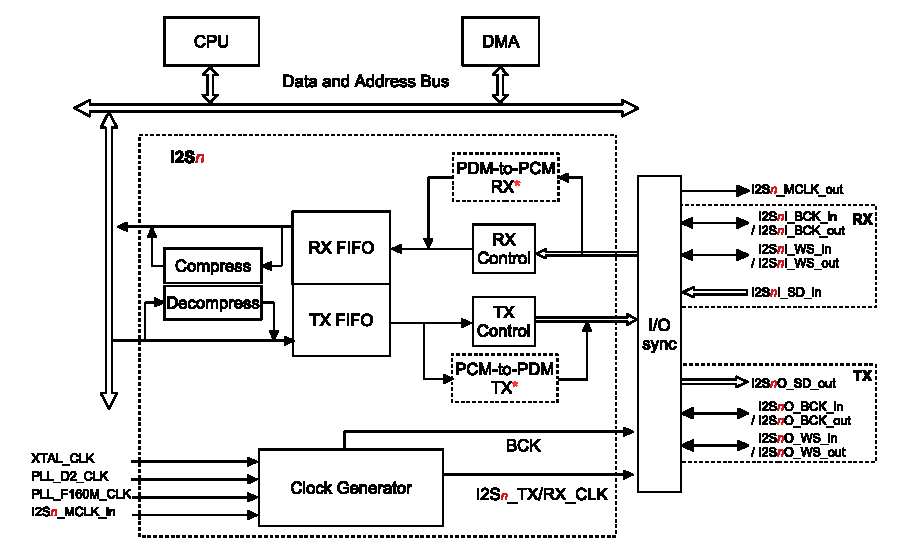
\includegraphics[width=0.9\textwidth]{03-I2S/figures/i2s_arch_20220729.eps}}\\
    注:图中 PDM-to-PCM RX 和 PCM-to-PDM TX 仅适用于 I2S\regindex{0}。
    \caption{\chipname{} I2S 系统框图}
    \label{Figure:i2s_arch}
\end{figure}

图 \ref{Figure:i2s_arch} 是 \chipname{} I2S\regindex{n} 模块的结构框图。\chipname{} I2S\regindex{n} 模块包含:
\begin{itemize}
    \item 独立的发送单元 (TX control)
    \item 独立的接收单元 (RX control)
    \item 输入输出时序调节单元 (I/O sync)
    \item 时钟分频器 (Clock Generator)
    \item 64 x 32-bit TX FIFO
    \item 64 x 32-bit RX FIFO
    \item 压缩/解压缩模块 (Compress/Decompress)
\end{itemize}
\chipname{} I2S\regindex{n} 模块支持 GDMA,可访问内部存储器和外部存储器,更多信息见章节 \ref{mod:dma} \textit{\nameref{mod:dma}}。


发送单元和接收单元各自有一组三线接口,分别为串行时钟线 BCK,字选择线 WS 和串行数据线 SD。其中,发送单元的 SD 线固定为输出,接收单元的 SD 线固定为接收。发送单元和接收单元的 BCK 和 WS 信号线均可配置为主机输出模式或从机输入模式。



图 \ref{Figure:i2s_arch} 右侧为 I2S\regindex{n} 模块的信号总线。RX 和 TX 模块的信号命名规则为:I2S\regindex{n}\textcolor{red}{A}\_\textcolor{red}{B}\_\textcolor{red}{C},例如 I2S\regindex{n}\textcolor{red}{I}\_\textcolor{red}{BCK}\_\textcolor{red}{in}。其中:

\begin{itemize}
    \item ``A" 表示 I2S 模块的数据总线的方向
    \begin{itemize}
        \item ``I" 表示输入
        \item ``O" 表示输出
    \end{itemize}
    \item ``B" 表示信号功能,包括:
    \begin{itemize}
        \item 串行时钟信号 (BCK)
        \item 字选择信号 (WS)
        \item 串行数据信号 (SD)
    \end{itemize}
    \item ``C" 表示该信号的方向
    \begin{itemize}
        \item ``in" 表示该信号输入 I2S\regindex{n} 模块
        \item ``out" 表示该信号自 I2S\regindex{n} 模块输出
    \end{itemize}
\end{itemize}

I2S\regindex{n} 各信号的具体描述见表 \ref{table:I2S 信号总线描述}。


\begin{table}[H]
    \centering
    \caption{模块信号描述}
    \label{table:I2S 信号总线描述}
    \begin{threeparttable}
    \begin{tabular}{|p{3cm}|p{1.5cm}|p{8cm}| }
    \hline
    \rowcolor{lightgray}
    \textbf{信号\tnote{*}}&\textbf{方向}&\textbf{功能}\\
    \hline
    I2S\regindex{n}I\_BCK\_in & 输入 & 从机模式下,输入 BCK 信号,用于 RX 模块\\
    \hline
    I2S\regindex{n}I\_BCK\_out& 输出 & 主机模式下,输出 BCK 信号,用于 RX 模块\\
    \hline
    I2S\regindex{n}I\_WS\_in & 输入 & 从机模式下,输入 WS 信号,用于 RX 模块\\
    \hline
    I2S\regindex{n}I\_WS\_out& 输出 & 主机模式下,输出 WS 信号,用于 RX 模块\\\hline
    I2S\regindex{n}I\_Data\_in& 输入 & RX 模块 的串行输入数据线\\\hline
    I2S\regindex{n}O\_Data\_out& 输出 & TX 模块 的串行输出数据线\\\hline
    I2S\regindex{n}O\_BCK\_in& 输入 & 从机模式下,输入 BCK 信号,用于 TX 模块 \\\hline
    I2S\regindex{n}O\_BCK\_out& 输出 & 主机模式下,输出 BCK 信号,用于 TX 模块 \\\hline
    I2S\regindex{n}O\_WS\_in& 输入 & 从机模式下,输入 WS 信号,用于 TX 模块\\\hline
    I2S\regindex{n}O\_WS\_out& 输出 & 主机模式下,输出 WS 信号,用于 TX 模块\\\hline
    I2S\regindex{n}\_MCLK\_in& 输入 & 从机模式下,来自外部芯片的时钟源\\\hline
    I2S\regindex{n}\_MCLK\_out& 输出 & 主机模式下,作为外部芯片的时钟源\\\hline
    I2S\regindex{0}I\_Data1\_in& 输入 & RX 模块 在 PDM-to-PCM 模式下的串行输入数据线\\\hline
    I2S\regindex{0}I\_Data2\_in& 输入 & RX 模块 在 PDM-to-PCM 模式下的串行输入数据线\\\hline
    I2S\regindex{0}I\_Data3\_in& 输入 & RX 模块 在 PDM-to-PCM 模式下的串行输入数据线\\\hline
    I2S\regindex{0}O\_Data1\_out& 输出 & TX 模块 在 PCM-to-PDM 模式下的串行输出数据线\\\hline
    \end{tabular}
    \begin{tablenotes}
            \item[*] I2S\regindex{n} 的所有信号均需要经过 GPIO 交换矩阵映射到芯片的管脚。更多信息请参考章节 \ref{mod:iomuxgpio} \textit{\nameref{mod:iomuxgpio}}。
    \end{tablenotes}
    \end{threeparttable}
\end{table}



\section{I2S\regindex{n} 模块支持的音频协议} \label{I2S_supported_protocal}

\chipname{} I2S\regindex{n} 模块支持多种音频标准,包括 TDM Philips 标准、TDM MSB 对齐标准、TDM PCM 标准以及 PDM 标准。

用户可通过配置以下寄存器,选择所需的音频标准:
\begin{itemize}
    \item \hyperref[fielddesc:I2SRXMSBSHIFT]{I2S\regindex{n}\_TX/RX\_TDM\_EN}
    \begin{itemize}
        \item 0:禁用 TDM 模式
        \item 1:选择 TDM 模式
    \end{itemize}
    \item \hyperref[fielddesc:I2SRXMSBSHIFT]{I2S\regindex{n}\_TX/RX\_PDM\_EN}
    \begin{itemize}
        \item 0:禁用 PDM 模式
        \item 1:选择 PDM 模式
    \end{itemize}
    \hyperref[fielddesc:I2SRXMSBSHIFT]{I2S\regindex{n}\_TX/RX\_MSB\_SHIFT}
    \begin{itemize}
        \item 0:配置 WS 信号和 SD 信号同时开始变化,即选择 MSB 对齐标准
        \item 1:配置 WS 信号先于 SD 信号一个 BCK 时钟周期开始变化,即选择 Philips 标准或 PCM 标准
    \end{itemize}
    \item \hyperref[fielddesc:I2SRXPCMBYPASS]{I2S\regindex{n}\_TX/RX\_PCM\_BYPASS}
    \begin{itemize}
        \item 0:选择 PCM 标准
        \item 1:禁用 PCM 标准
    \end{itemize}
\end{itemize}

\subsection{TDM Philips 标准模式}

在 Philips 标准下,在 BCK 的下降沿,WS 信号先于 SD 信号一个 BCK 时钟周期开始变化,即 WS 信号从当前通道数据的第一个位之前的一个时钟开始有效,并在当前通道数据发送结束前一个 BCK 时钟周期开始变化。SD 信号线上首先传输音频数据的最高位。

与 Philips 标准相比,TDM Philips 标准支持更多的通道,见图 \ref{Figure:i2s_phillips_standard}。
\begin{figure}[H]
    \centering
    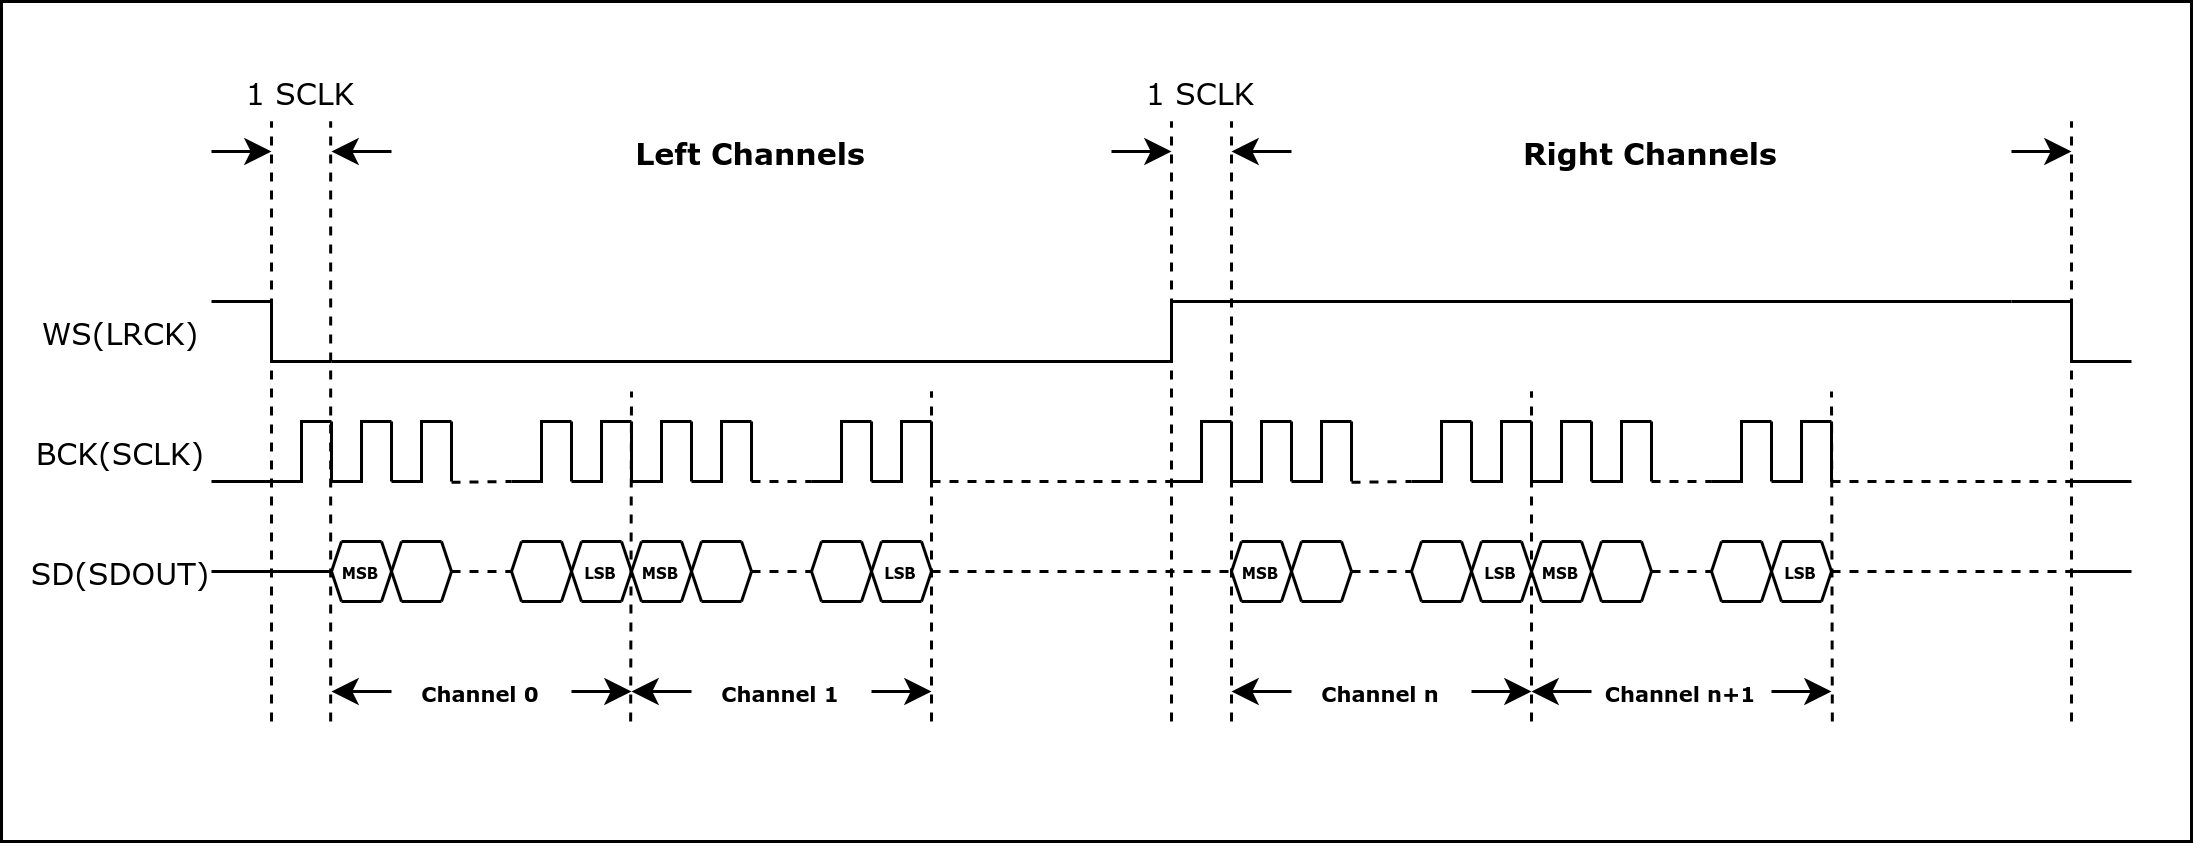
\includegraphics[width=1.0\textwidth]{03-I2S/figures/i2s_tdm_phillips_mode.png}
    \caption{时序图 -- TDM Philips 标准}
    \label{Figure:i2s_phillips_standard}
\end{figure}

\subsection{TDM MSB 对齐标准模式}

MSB 对齐标准下,在 BCK 下降沿,WS 信号和 SD 信号同时变化。WS 持续到当前通道数据发送结束,SD 信号线上首先传输音频数据的最高位。

与 MSB 对齐标准相比,TDM MSB 对齐标准支持更多的通道,见图 \ref{Figure:i2s_MSB_32_mode}。

\begin{figure}[H]
    \centering
    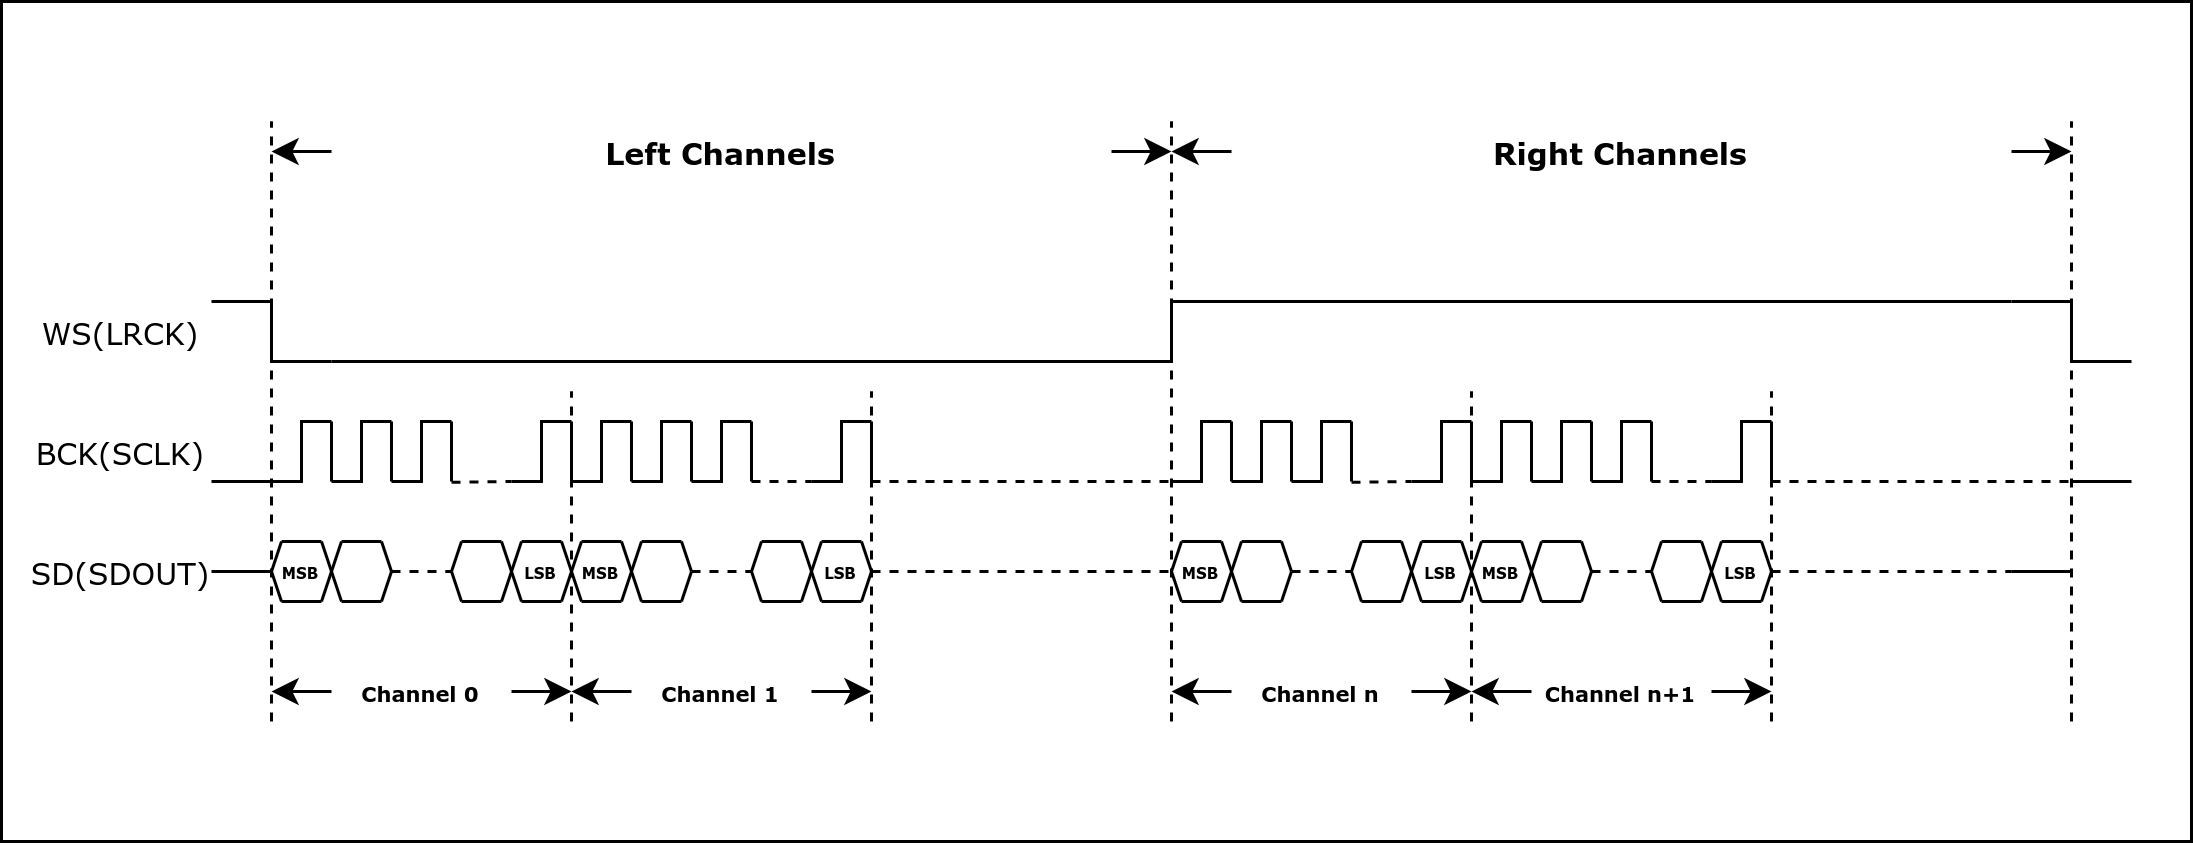
\includegraphics[width=1.0\textwidth]{03-I2S/figures/i2s_tdm_msb_mode.png}
    \caption{时序图 -- TDM MSB 对齐标准}
    \label{Figure:i2s_MSB_32_mode}
\end{figure}

%用户可清零 \hyperref[fielddesc:I2SRXMSBSHIFT]{I2S\_RX\_MSB\_SHIFT} 和 \hyperref[fielddesc:I2STXMSBSHIFT]{I2S\_TX\_MSB\_SHIFT},使能 I2S 模块在接收数据和发送数据时处于 TDM MSB 对齐标准模式。

\subsection{TDM PCM 标准模式}

在 PCM 标准的短帧同步模式下,在 BCK 的下降沿,WS 信号先于 SD 信号一个 BCK 时钟周期开始变化,即 WS 信号从当前通道数据的第一个位之前的一个时钟开始有效,并持续一个 BCK 时钟周期。SD 信号线上首先传输音频数据的最高位。

与 PCM 标准相比,TDM PCM 标准支持更多的通道,见图 \ref{Figure:i2s_pcm_mode} 所示。

\begin{figure}[H]
    \centering
    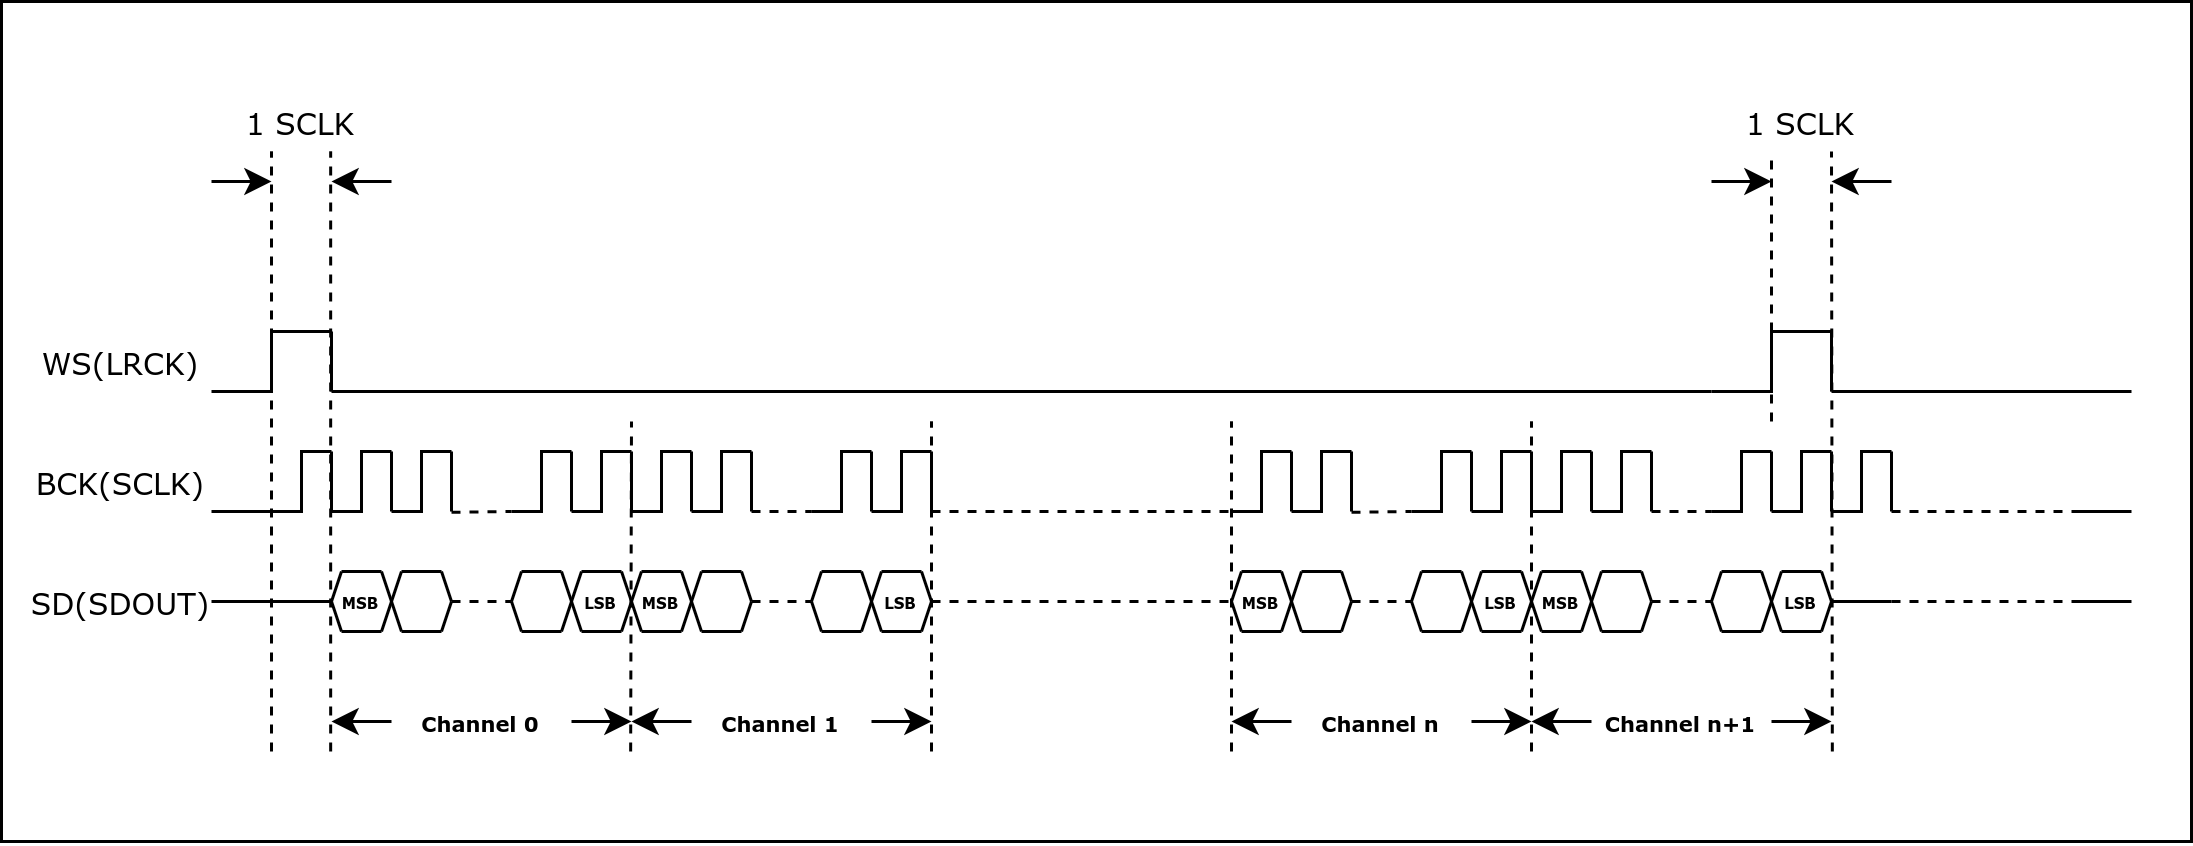
\includegraphics[width=1.0\textwidth]{03-I2S/figures/i2s_tdm_pcm_mode.png}
    \caption{时序图 -- TDM PCM 标准}
    \label{Figure:i2s_pcm_mode}
\end{figure}

%如果 \hyperref[fielddesc:I2SRXMSBSHIFT]{I2S\_RX\_MSB\_SHIFT} 和 \hyperref[fielddesc:I2STXMSBSHIFT]{I2S\_TX\_MSB\_SHIFT} 置 1,那么 I2S 模块接收数据和发送数据将使用短帧同步模式。

\subsection{PDM 标准模式}
如图 \ref{Figure:i2s_pdm_mode} 所示,在 PDM 标准下,WS 代表左/右声道,在 BCK 的下降沿,WS 与 SD 同时变化。WS 在数据发送过程中持续变化,WS 的高低对应两个声道。%SD 信号线上首先传输音频数据的最高位。

\begin{figure}[H]
    \centering
    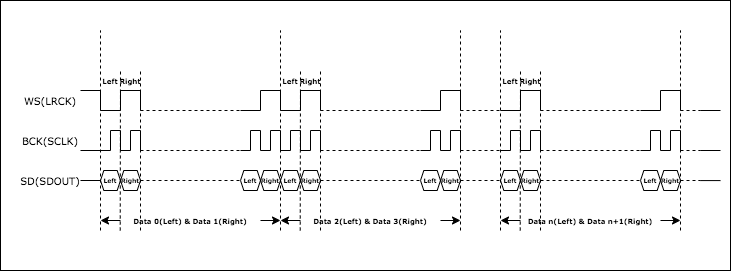
\includegraphics[width=1.0\textwidth]{03-I2S/figures/i2s_pdm_mode.png}
    \caption{时序图 -- PDM 标准}
    \label{Figure:i2s_pdm_mode}
\end{figure}

\section{TX/RX 模块时钟}\label{The Clock of I2S Module}

I2S\regindex{n}\_TX/RX\_CLK 作为 I2S\regindex{n} TX/RX 模块的主时钟,可由以下时钟分频所得(见图 \ref{Figure:i2s_clk}):
\begin{itemize}
    \item 40 MHz XTAL\_CLK
    \item 160 MHz PLL\_F160M\_CLK
    \item 240 MHz PLL\_D2\_CLK
    \item 或外部输入时钟:I2S\regindex{n}\_MCLK\_in
\end{itemize}

\hyperref[fielddesc:I2SRXCLKSEL]{I2S\regindex{n}\_TX/RX\_CLK\_SEL} 用于选择 I2S\regindex{n} TX/RX 的时钟源,\hyperref[fielddesc:I2SRXCLKACTIVE]{I2S\regindex{n}\_TX/RX\_CLK\_ACTIVE} 用于使能或者关闭 I2S\regindex{n} TX/RX 模块的时钟源。
%由 40 MHz 的 XTAL\_40M\_CLK 时钟, 160 MHz 的 PLL\_160M\_CLK 时钟, 240 MHz 的 PLL\_240M\_CLK 时钟或者外部输入时钟 I2S\_MCLK\_in 进行分频获得。
%I2S\regindex{n} TX/RX 模块的串行时钟 BCK 再由 I2S\regindex{n}\_TX/RX\_CLK 分频获得,如图 \ref{Figure:i2s_clk} 所示。\hyperref[fielddesc:I2SRXCLKSEL]{I2S\regindex{n}\_TX/RX\_CLK\_SEL} 用于选择 I2S\regindex{n} TX/RX 的时钟源,\hyperref[fielddesc:I2SRXCLKACTIVE]{I2S\regindex{n}\_TX/RX\_CLK\_ACTIVE} 用于使能或者关闭 I2S\regindex{n} TX/RX 模块的时钟源。

\begin{figure}[H]
    \centering
    \fbox{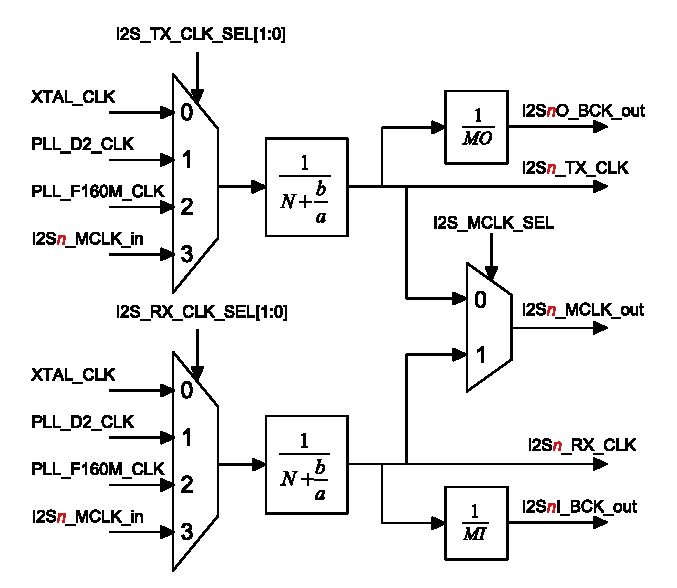
\includegraphics[width=0.6\textwidth]{03-I2S/figures/i2s_clk_20220729}}
    \caption{I2S\regindex{n} 时钟}
    \label{Figure:i2s_clk}
\end{figure}

I2S\regindex{n}\_TX/RX\_CLK 的频率 $f_{\textrm{I2S\regindex{n}\_TX/RX\_CLK}}$ 与分频器时钟源频率 $f_{\textrm{I2S\regindex{n}\_CLK\_S}}$ 间的关系如下:
$$f_{\textrm{I2S\regindex{n}\_TX/RX\_CLK}}=\frac{f_{\textrm{I2S\regindex{n}\_CLK\_S}}}{\textrm{N} + \frac{\textrm{b}}{\textrm{a}}}$$

其中, 2 =< N <= 256,N 对应为 \hyperref[regdesc:I2STXCLKMCONFREG]{I2S\regindex{n}\_TX/RX\_CLKM\_CONF\_REG} 寄存器中 \hyperref[fielddesc:I2STXCLKMDIVNUM]{I2S\regindex{n}\_TX/RX\_CLKM\_DIV\_NUM} 的值,具体为:

\begin{itemize}
    \item \hyperref[fielddesc:I2STXCLKMDIVNUM]{I2S\regindex{n}\_TX/RX\_CLKM\_DIV\_NUM} = 0 时,N = 256;
    \item \hyperref[fielddesc:I2STXCLKMDIVNUM]{I2S\regindex{n}\_TX/RX\_CLKM\_DIV\_NUM} = 1 时,N = 2;
    \item \hyperref[fielddesc:I2STXCLKMDIVNUM]{I2S\regindex{n}\_TX/RX\_CLKM\_DIV\_NUM} 为其它值时,N = \hyperref[fielddesc:I2STXCLKMDIVNUM]{I2S\regindex{n}\_TX/RX\_CLKM\_DIV\_NUM} 的值。

\end{itemize}

分数部分分频系数 a、b 唯一对应系数 x、y、z、yn1。系数对应公式为:
\begin{itemize}
    \item 当 $\textrm{b} <= \frac{\textrm{a}}{2}$ 时,$\textrm{yn1} = 0$,$\textrm{x} = floor([\frac{\textrm{a}}{\textrm{b}}]) - 1$,$\textrm{y} = \textrm{a}\%\textrm{b}$,$\textrm{z} = \textrm{b}$;
    \item 当 $\textrm{b} > \frac{\textrm{a}}{2}$ 时,$\textrm{yn1}=1$,$\textrm{x} = floor([\frac{\textrm{a}}{\textrm{a - b}}]) - 1$,$\textrm{y} = \textrm{a}\%\textrm{(a - b)}$,$\textrm{z}=\textrm{a - b}$;
\end{itemize}

系数 x、y、z、yn1 在 \hyperref[fielddesc:I2STXCLKMDIVX]{I2S\regindex{n}\_TX/RX\_CLKM\_DIV\_X}、\hyperref[fielddesc:I2STXCLKMDIVY]{I2S\regindex{n}\_TX/RX\_CLKM\_DIV\_Y}、\hyperref[fielddesc:I2STXCLKMDIVZ]{I2S\regindex{n}\_TX/RX\_CLKM\_DIV\_Z}、\hyperref[fielddesc:I2STXCLKMDIVYN1]{I2S\regindex{n}\_TX/RXCLKM\_DIV\_YN1} 中配置。 \\
对于整数分频,\hyperref[fielddesc:I2STXCLKMDIVX]{I2S\regindex{n}\_TX/RX\_CLKM\_DIV\_X} 和 \hyperref[fielddesc:I2STXCLKMDIVZ]{I2S\regindex{n}\_TX/RX\_CLKM\_DIV\_Z} 清零,\hyperref[fielddesc:I2STXCLKMDIVY]{I2S\regindex{n}\_TX/RX\_CLKM\_DIV\_Y} 置为 1。

\begin{tiplisting}
使用小数分频功能可能会产生时钟抖动。
\end{tiplisting}

I2S\regindex{n} TX/RX 模块的串行时钟 BCK 再由 I2S\regindex{n}\_TX/RX\_CLK 分频获得,如图 \ref{Figure:i2s_clk} 所示。

在主机发送模式下,I2S\regindex{n} TX 模块的串行时钟 BCK 为 I2S\regindex{n}O\_BCK\_out 信号,由 I2S\regindex{n}\_TX\_CLK 分频获得。即:

$$f_{\textrm{I2S\regindex{n}O\_BCK\_out}} = \frac{f_{\textrm{I2S\regindex{n}\_TX\_CLK}}}{\textrm{MO}}$$


其中,MO 的值为 \hyperref[fielddesc:I2STXBCKDIVNUM]{I2S\regindex{n}\_TX\_BCK\_DIV\_NUM} 的值 + 1,即:
$$ \textrm{MO} = \textrm{\hyperref[fielddesc:I2STXBCKDIVNUM]{I2S\regindex{n}\_TX\_BCK\_DIV\_NUM}} + 1 $$

{\bfseries 注意:}

\hyperref[fielddesc:I2STXBCKDIVNUM]{I2S\regindex{n}\_TX\_BCK\_DIV\_NUM} 不可配置为 1。

在主机接收模式下,I2S\regindex{n} RX 模块的串行时钟 BCK 为 I2S\regindex{n}I\_BCK\_out 信号,由 I2S\regindex{n}\_RX\_CLK 分频获得。即:

$$f_{\textrm{I2S\regindex{n}I\_BCK\_out}} = \frac{f_{\textrm{I2S\regindex{n}\_RX\_CLK}}}{\textrm{MI}}$$

其中 MI 对应 \hyperref[fielddesc:I2SRXBCKDIVNUM]{I2S\regindex{n}\_RX\_BCK\_DIV\_NUM} 的值 + 1,即:
$$ \textrm{MI} = \textrm{\hyperref[fielddesc:I2STXBCKDIVNUM]{I2S\regindex{n}\_RX\_BCK\_DIV\_NUM}} + 1 $$


{\bfseries 注意:}
\begin{itemize}
    \item \hyperref[fielddesc:I2SRXBCKDIVNUM]{I2S\regindex{n}\_RX\_BCK\_DIV\_NUM} 不可配置为 1;
    \item 当模块处于从机模式时,必须保证 $f_{\textrm{I2S\regindex{n}\_TX/RX\_CLK}}$ >= 8 * $f_{\textrm{BCK}}$。另外模块可以输出 I2S\regindex{n}\_MCLK\_out 作为外部设备的主时钟。

\end{itemize}

\section{I2S\regindex{n} 模块复位} \label{i2s_module_reset}

I2S\regindex{n} 模块中各个单元以及 FIFO 可通过配置相关位进行复位:
\begin{itemize}
\item I2S\regindex{n} TX/RX 单元:可配置 \hyperref[fielddesc:I2STXRESET]{I2S\regindex{n}\_TX\_RESET} 和 \hyperref[fielddesc:I2SRXRESET]{I2S\regindex{n}\_RX\_RESET} 位进行复位;
\item I2S\regindex{n} TX/RX FIFO:可配置 \hyperref[fielddesc:I2STXFIFORESET]{I2S\regindex{n}\_TX\_FIFO\_RESET} 和 \hyperref[fielddesc:I2SRXFIFORESET]{I2S\regindex{n}\_RX\_FIFO\_RESET} 位进行复位。
\end{itemize}


{\bfseries 注意:}
在模块和 FIFO 复位之前,需要先配置 I2S\regindex{n} 模块时钟。


\section{I2S\regindex{n} 主/从机模式}

\chipname{} I2S\regindex{n} 模块可作为主机或从机。用户可配置  \hyperref[fielddesc:I2STXSLAVEMOD]{I2S\regindex{n}\_TX\_SLAVE\_MOD} 和 \hyperref[fielddesc:I2SRXSLAVEMOD]{I2S\regindex{n}\_RX\_SLAVE\_MOD} 选择需要的模式。

\begin{itemize}
    \item \hyperref[fielddesc:I2STXSLAVEMOD]{I2S\regindex{n}\_TX\_SLAVE\_MOD}
    \begin{itemize}
        \item 0:主机发送模式
        \item 1:从机发送模式
    \end{itemize}
    \item \hyperref[fielddesc:I2SRXSLAVEMOD]{I2S\regindex{n}\_RX\_SLAVE\_MOD}
    \begin{itemize}
        \item 0:主机接收模式
        \item 1:从机接收模式
    \end{itemize}
\end{itemize}

\subsection{主/从机发送模式} \label{subsubsection:master/slave_transmitting_mode}
\begin{itemize}
    \item 主机发送模式
    \begin{itemize}
        \item 置位 \hyperref[fielddesc:I2STXSTART]{I2S\regindex{n}\_TX\_START} 位启动一次发送操作。
        \item 置位该位,发送单元会一直输出时钟信号和串行数据。
        \item 置位 \hyperref[fielddesc:I2STXSTOPEN]{I2S\regindex{n}\_TX\_STOP\_EN} 时,如果 FIFO 中的数据全部发送完毕,则主机停止发送数据。
        \item 清零 \hyperref[fielddesc:I2STXSTOPEN]{I2S\regindex{n}\_TX\_STOP\_EN} 时,如果 FIFO 中的数据全部发送完毕,并且没有新数据填入,发送模块将一直发送最后一帧数据。
        \item 当 \hyperref[fielddesc:I2STXSTART]{I2S\regindex{n}\_TX\_START} 位被清零时,主机停止发送数据。
    \end{itemize}
    \item 从机发送模式
     \begin{itemize}
        \item 置位 \hyperref[fielddesc:I2STXSTART]{I2S\regindex{n}\_TX\_START}。
        \item 发送单元等待主机 BCK 时钟,来启动发送操作。
        \item 置位 \hyperref[fielddesc:I2STXSTOPEN]{I2S\regindex{n}\_TX\_STOP\_EN} 时,如果 FIFO 中的数据全部发送完毕,则从机发送数据一直为零,直到主机停止发送 BCK 时钟为止。
        \item 清零 \hyperref[fielddesc:I2STXSTOPEN]{I2S\regindex{n}\_TX\_STOP\_EN} 时,如果 FIFO 中的数据全部发送完毕,并且没有新数据填入,发送单元将一直发送最后一帧数据。
        \item 当 \hyperref[fielddesc:I2STXSTART]{I2S\regindex{n}\_TX\_START} 位被清零时,从机发送数据一直为零,直到主机停止发送 BCK 时钟为止。
    \end{itemize}
\end{itemize}

\subsection{主/从机接收模式}
\begin{itemize}
    \item 主机接收模式
    \begin{itemize}
        \item 置位 \hyperref[fielddesc:I2SRXSTART]{I2S\regindex{n}\_RX\_START} 启动一次接收操作。
        \item 接收单元会一直输出时钟信号,并对输入数据进行采样。
        \item 清零 \hyperref[fielddesc:I2SRXSTART]{I2S\regindex{n}\_RX\_START},接收单元停止接收数据。
    \end{itemize}
    \item 从机接收模式
     \begin{itemize}
        \item 置位 \hyperref[fielddesc:I2SRXSTART]{I2S\regindex{n}\_RX\_START}。
        \item 等待主机 BCK 时钟,来启动接收操作。
        \item 清零 \hyperref[fielddesc:I2SRXSTART]{I2S\regindex{n}\_RX\_START},接收单元停止接收数据。
    \end{itemize}
\end{itemize}

\section{发送数据}\label{TXCHAN}

\begin{tiplisting}
本小节以及后续小节所述的配置,均需要通过置位 \hyperref[fielddesc:I2STXUPDATE]{I2S\regindex{n}\_TX\_UPDATE} 的方式来进行更新,从而将 I2S\regindex{n} TX 寄存器数据从 APB 时钟域同步到 I2S\regindex{n} TX 时钟域。详细配置见第 \ref{sec:configure-i2s-as-tx-mode} 小节。
\end{tiplisting}
\vspace{-2em}
\chipname{} I2S\regindex{n} 发送数据时,从 DMA 读取数据,经过数据格式控制和通道模式控制,从外设输出信号输出对应数据。
\subsection{数据格式控制}
数据格式控制分为三个阶段:
\begin{itemize}
    \item 第一阶段从内存中读出有效数据并写入 TX FIFO;
    \item 第二阶段将待发送数据从 TX FIFO 中读出,并进行输出数据模式转换;
    \item 第三阶段,将待发送数据转换为串行数据流输出。
\end{itemize}

\subsubsection{通道有效数据位宽}
\hyperref[fielddesc:I2STXBITSMOD]{I2S\regindex{n}\_TX\_BITS\_MOD} 和 \hyperref[fielddesc:I2STX24FILLEN]{I2S\regindex{n}\_TX\_24\_FILL\_EN} 决定了每个通道的有效数据位宽,其可取值和对应的有效数据位宽如下表:

\begin{table}[H]
    \centering
    \caption{通道有效数据位宽控制}
    \label{table:TX_BITS_MODE}
    \begin{threeparttable}
    \begin{tabular}{|p{4.2cm}|R{3.1cm}|R{3.5cm}|}
    \hline
    \rowcolor{lightgray}
    \textbf{通道有效数据位宽} & \textbf{\hyperref[fielddesc:I2STXBITSMOD]{I2S\regindex{n}\_TX\_BITS\_MOD}}  & \textbf{\hyperref[fielddesc:I2STX24FILLEN]{I2S\regindex{n}\_TX\_24\_FILL\_EN}} \\ \hline
    \multirow{2}*{32} & 31 & x\tnote{1} \\\cline{2-3}
                      & 23 & 1 \\\hline

                24    & 23 & 0 \\\hline

                16     & 15 & x \\\hline
                8     & 7 & x \\\hline
    \end{tabular}
            \begin{tablenotes}
            \item[1] 该值被忽略。
        \end{tablenotes}

    \end{threeparttable}
\end{table}

\subsubsection{通道有效数据字节序}
I2S\regindex{n} 通过 DMA 读取数据之后,\hyperref[fielddesc:I2STXBIGENDIAN]{I2S\regindex{n}\_TX\_BIG\_ENDIAN} 用于控制从 DMA 读取数据的字节序。下表描述了不同通道有效数据位宽下,该寄存器对读取数据的控制。

\begin{table}[H]
    \centering
    \caption{通道有效数据字节序控制}
    \label{tab:byte-order-control-of-valid-data}
    \begin{tabular}{|p{3.2cm}|p{2.7cm}|p{3.2cm}|R{3.5cm}|}
    \hline
    \rowcolor{lightgray}
    \textbf{通道有效数据位宽} & \textbf{原始数据}  & \textbf{控制后数据}  & \textbf{\hyperref[fielddesc:I2STXBIGENDIAN]{I2S\regindex{n}\_TX\_BIG\_ENDIAN}} \\ \hline
    \multirow{2}*{32} & \multirow{2}*{\{B3, B2, B1, B0\}} & \{B3, B2, B1, B0\} & 0 \\\cline{3-4}
                      && \{B0, B1, B2, B3\} & 1 \\\hline

    \multirow{2}*{24} & \multirow{2}*{\{B2, B1, B0\}} & \{B2, B1, B0\} & 0 \\\cline{3-4}
                      && \{B0, B1, B2\} & 1 \\\hline

    \multirow{2}*{16} & \multirow{2}*{\{B1, B0\}} & \{B1, B0\} & 0 \\\cline{3-4}
                      && \{B0, B1\} & 1 \\\hline

                8     & \{B0\} & \{B0\} & x \\\hline
    \end{tabular}
\end{table}

\subsubsection{A 率/$\mu$ 率压缩/解压缩}
\chipname{} I2S\regindex{n} 对排列好字节序的有效数据会按照 32-bit(缺省高位补 0$^*$)的方式进行 A 率/$\mu$ 率压缩/解压缩。
\begin{tiplisting}
缺省高位补 0,即如果有效数据位宽小于 32,则待压缩/解压缩数据的 [31: 有效位宽] 位自动填充 0。
\end{tiplisting}

配置 \hyperref[fielddesc:I2STXPCMBYPASS]{I2S\regindex{n}\_TX\_PCM\_BYPASS} 为:
\begin{itemize}
\item 0,则不进行压缩/解压缩
\item 1,则进行压缩/解压缩
\end{itemize}
配置 \hyperref[fielddesc:I2STXPCMCONF]{I2S\regindex{n}\_TX\_PCM\_CONF} 为:
\begin{itemize}
\item 0,A 律解压缩
\item 1,A 律压缩
\item 2,$\mu$ 律解压缩
\item 3,$\mu$ 律压缩
\end{itemize}
至此,数据格式控制的第一阶段完成。

\subsubsection{通道发送数据位宽}
\chipname{} I2S\regindex{n} 中,\hyperref[fielddesc:I2STXTDMCHANBITS]{I2S\regindex{n}\_TX\_TDM\_CHAN\_BITS} 决定了每个通道发送数据的位宽。

\begin{itemize}
\item 当每个通道发送数据的位宽大于有效数据位宽时,会在剩余的位置补充 0。此时,配置 \hyperref[fielddesc:I2STXLEFTALIGN]{I2S\regindex{n}\_TX\_LEFT\_ALIGN} 为:
\begin{itemize}
\item 0,有效数据位于发送数据低位。
\item 1,有效数据位于发送数据高位。
\end{itemize}
\item 当每个通道发送数据的位宽小于有效数据位宽时,每次发送数据仅发送低位有效数据部分,高位部分将被舍弃。
\end{itemize}
至此,数据格式控制的第二阶段完成。

\subsubsection{通道数据比特顺序}
\chipname{} I2S\regindex{n} 通道数据比特顺序由 \hyperref[fielddesc:I2STXBITORDER]{I2S\regindex{n}\_TX\_BIT\_ORDER} 控制:
\begin{itemize}
\item 1,数据从低位向高位依次发送。
\item 0,数据从高位向低位依次发送。
\end{itemize}
至此,数据格式控制部分全部完成。图 \ref{Figure:i2s_data_mode_control} 所示即为一次完整的 TX 数据格式控制过程。


\begin{figure}[H]
    \centering
    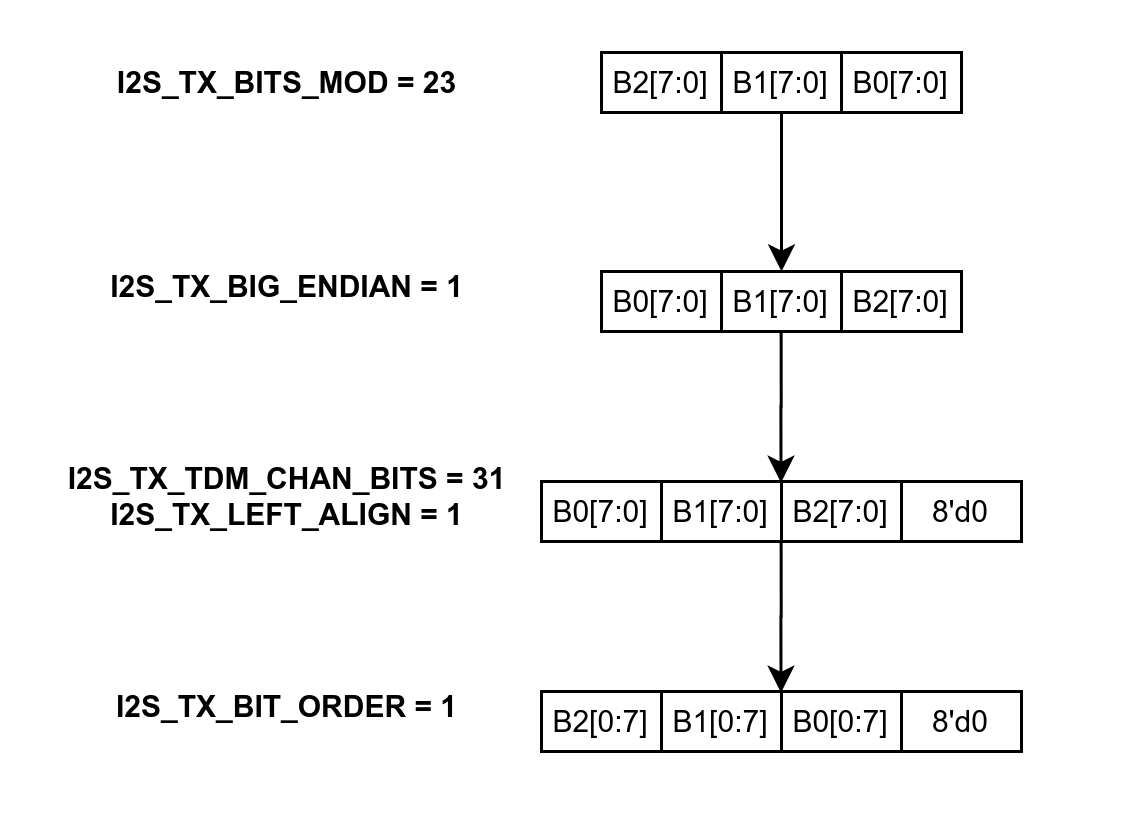
\includegraphics[width=0.8\textwidth]{03-I2S/figures/i2s_tx_data_config.png}
    \caption{TX 数据格式控制}
    \label{Figure:i2s_data_mode_control}
\end{figure}


\subsection{通道模式控制}
\chipname{} I2S\regindex{n} 支持 TDM 和 PDM 两种发送模式。置位 \hyperref[fielddesc:I2STXTDMEN]{I2S\regindex{n}\_TX\_TDM\_EN} 则为 TDM 发送模式,置位 \hyperref[fielddesc:I2STXPDMEN]{I2S\regindex{n}\_TX\_PDM\_EN} 则为 PDM 发送模式。

\begin{tiplisting}
\vspace{-2em}
\begin{itemize}
    \item \hyperref[fielddesc:I2STXTDMEN]{I2S\regindex{n}\_TX\_TDM\_EN} 和 \hyperref[fielddesc:I2STXPDMEN]{I2S\regindex{n}\_TX\_PDM\_EN} 不能同时置位或同时清零。
    \item 将 I2S\regindex{n} 模块设置为 TDM 双通道模式,可实现控制大多数 I2S 双声道编解码器。
    \end{itemize}
\end{tiplisting}


\subsubsection{TDM 模式下 I2S\regindex{n} 通道模式} \label{sec:tdm-channel-mode}
在 TDM 模式下,I2S\regindex{n} 支持最多 16 通道数据输出。发送通道数由 \hyperref[fielddesc:I2STXTDMTOTCHANNUM]{I2S\regindex{n}\_TX\_TDM\_TOT\_CHAN\_NUM} 控制。例如,配置 \hyperref[fielddesc:I2STXTDMTOTCHANNUM]{I2S\regindex{n}\_TX\_TDM\_TOT\_CHAN\_NUM} 为 5,则六个通道(通道 0 \verb+~+ 5)将用于发送数据,见图
\ref{Figure:i2s_tdm_channel_control}。

在发送数据的通道中,如果其对应的 \hyperref[fielddesc:I2STXTDMCHAN0EN]{I2S\regindex{n}\_TX\_TDM\_CHAN{\textcolor{red}{n}}\_EN} 为:

\begin{itemize}
    \item 1,则该通道发送通道数据。
    \item 0,则该通道发送数据由 \hyperref[fielddesc:I2STXCHANEQUAL]{I2S\regindex{n}\_TX\_CHAN\_EQUAL} 控制,当该值为:
    \begin{itemize}
        \item 1,则发送上个通道的数据。
        \item 0,则发送 \hyperref[fielddesc:I2SSINGLEDATA]{I2S\regindex{n}\_SINGLE\_DATA} 的值。
    \end{itemize}
\end{itemize}
当 I2S\regindex{n} 处于主机 TDM 模式下,WS 信号由 \hyperref[fielddesc:I2STXWSIDLEPOL]{I2S\regindex{n}\_TX\_WS\_IDLE\_POL} 和 \hyperref[fielddesc:I2STXTDMWSWIDTH]{I2S\regindex{n}\_TX\_TDM\_WS\_WIDTH} 控制。其中,\hyperref[fielddesc:I2STXWSIDLEPOL]{I2S\regindex{n}\_TX\_WS\_IDLE\_POL} 的值为 WS 信号的默认电平,\hyperref[fielddesc:I2STXTDMWSWIDTH]{I2S\regindex{n}\_TX\_TDM\_WS\_WIDTH} 的值为在发送所有通道数据的过程中,WS 为默认电平的周期数。另外,\hyperref[fielddesc:I2STXHALFSAMPLEBITS]{I2S\regindex{n}\_TX\_HALF\_SAMPLE\_BITS} 的值乘以 2,即为一个 WS 周期对应的 BCK 周期数。

\textbf{TDM 通道配置示例}

在本示例中,寄存器的配置如下:

\begin{itemize}
    \item 配置 I2S\_TX\_TDM\_CHAN\_NUM 为 5,即选择使用通道 0 \verb+~+ 5 进行数据发送。
    \item 配置 I2S\_TX\_CHAN\_EQUAL 为 1,即如果相应通道的 I2S\_TX\_TDM\_CHAN\regindex{n}\_EN 被置位,则该通道将发送上一通道的数据。\regindex{n} = 0 \verb+~+ 5。
    \item 配置 I2S\_TX\_TDM\_CHAN0/2/5\_EN 为 1,即这些通道将用于发送通道数据。
    \item 配置 I2S\_TX\_TDM\_CHAN1/3/4\_EN 为 0,则这些通道将发送上一个通道的数据。
\end{itemize}

配置完成后,则数据将按下图方式进行发送。

\begin{figure}[H]
    \centering
    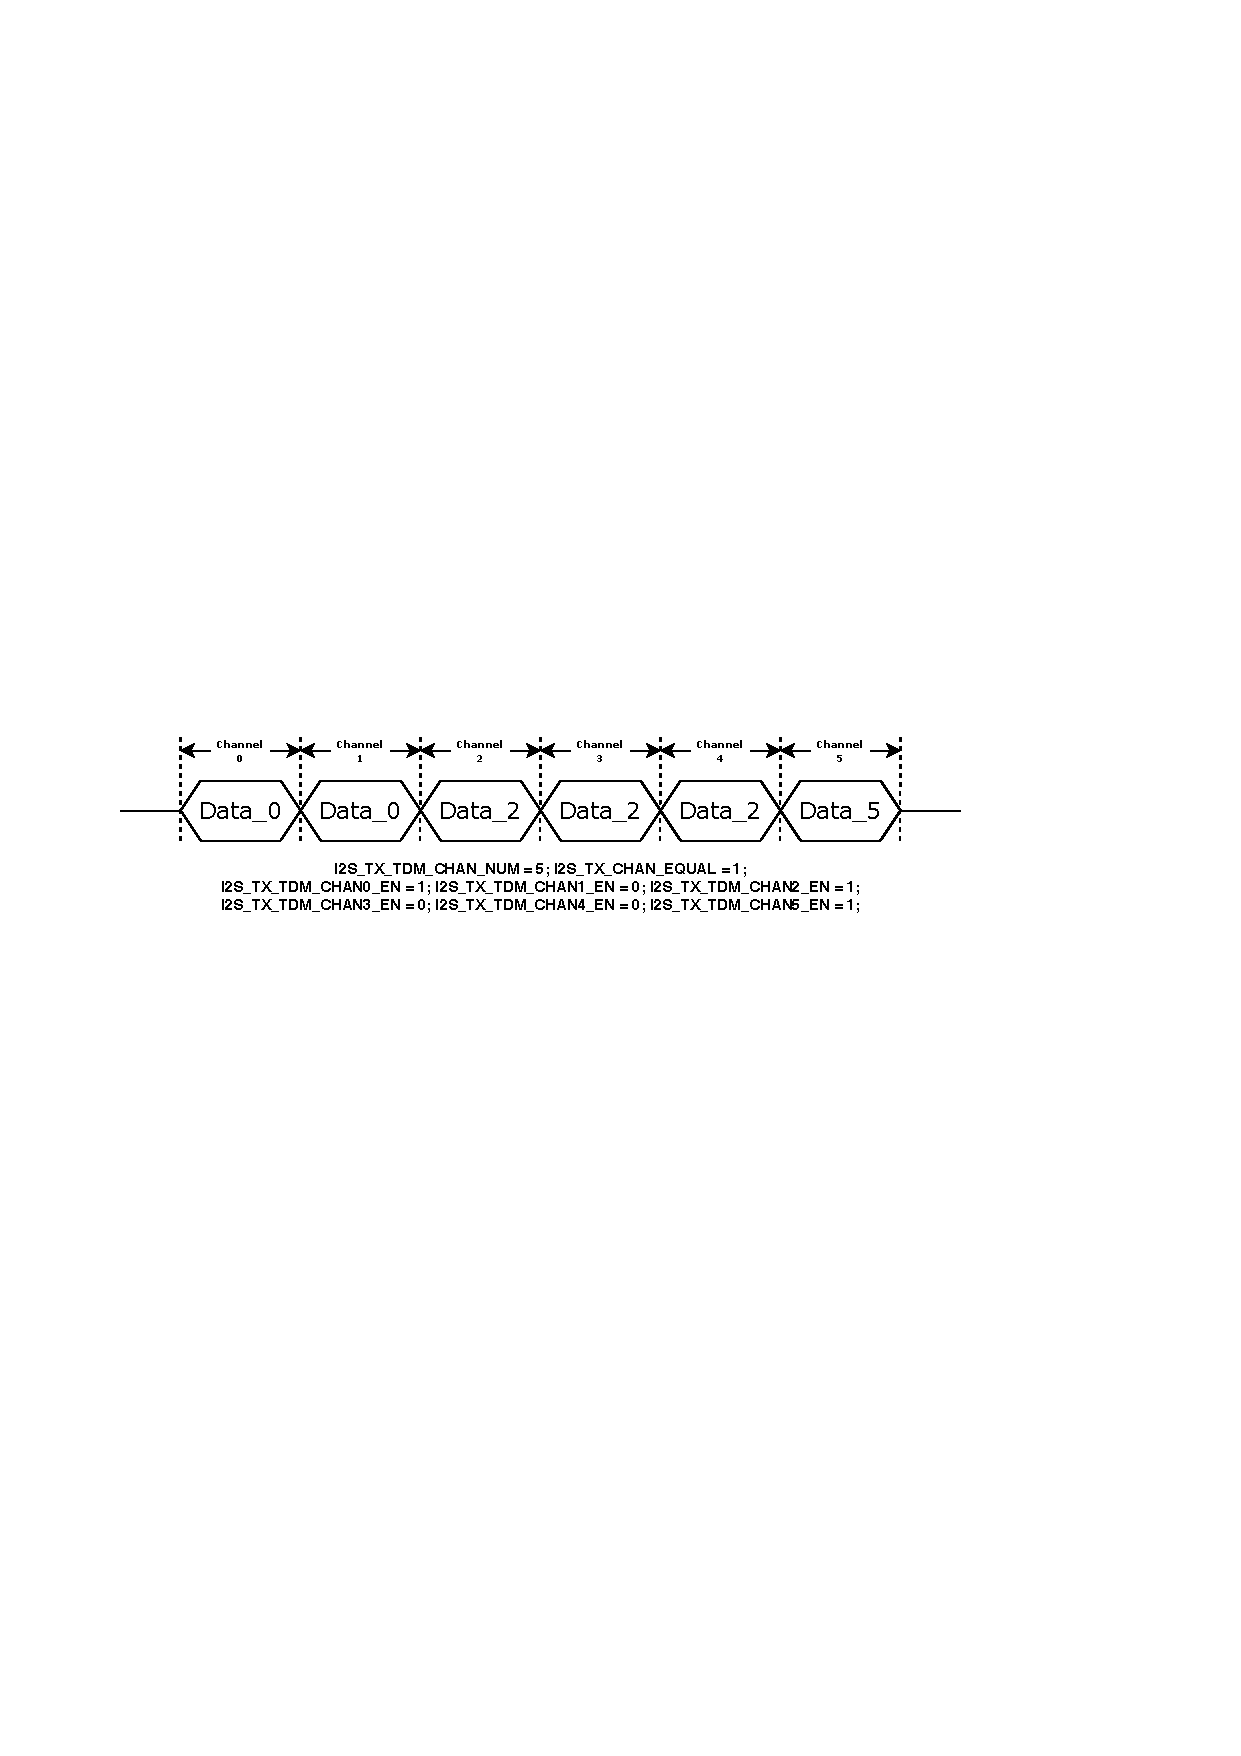
\includegraphics[width=1.0\textwidth]{03-I2S/figures/i2s_tdm_channel_config.pdf}
    \caption{TDM 通道控制}
    \label{Figure:i2s_tdm_channel_control}
\end{figure}


\subsubsection{PDM 模式下 I2S\regindex{n} 通道模式}
在 PDM 模式下,从 DMA 取得数据的过程由 \hyperref[fielddesc:I2STXMONO]{I2S\regindex{n}\_TX\_MONO} 和 \hyperref[fielddesc:I2STXMONOFSTVLD]{I2S\regindex{n}\_TX\_MONO\_FST\_VLD} 控制,具体如下表。请根据内存中存储的数据为单/双通道数据来配置该寄存器。

\begin{table}[H]
    \centering
    \caption{PDM 模式下 I2S\regindex{n} 取数逻辑}
    \label{table:TX_PDM_DATA_READ}
    \begin{tabular}{|p{6.6cm}|l|r|r|}
    \hline
    \rowcolor{lightgray}
    \textbf{取数逻辑} &\textbf{模式} &\textbf{\hyperref[fielddesc:I2STXMONO]{I2S\regindex{n}\_TX\_MONO}}  & \textbf{\hyperref[fielddesc:I2STXMONOFSTVLD]{I2S\regindex{n}\_TX\_MONO\_FST\_VLD}} \\ \hline
                        每个 WS 沿都向 DMA 发起取数请求 & 双声道 & 0 & x        \\ \hline
                        只在 WS 后半周期向 DMA 发起取数请求  & 单声道 & 1 & 0   \\ \hline
                        只在 WS 前半周期向 DMA 发起取数请求 & 单声道 & 1 & 1      \\ \hline
    \end{tabular}
\end{table}
在 PDM 模式下,I2S\regindex{n} 通道数据由 \hyperref[fielddesc:I2STXCHANMOD]{I2S\regindex{n}\_TX\_CHAN\_MOD} 和 \hyperref[fielddesc:I2STXWSIDLEPOL]{I2S\regindex{n}\_TX\_WS\_IDLE\_POL} 控制,具体如下表。

\begin{table}[H]
    \centering
    \caption{PDM 模式下 I2S\regindex{n} 通道模式控制}
    \label{table:TX_PDM_DATA}
    \begin{threeparttable}
    \begin{tabular}{|p{1.3cm}|L{4.7cm}|L{4.7cm}|R{2.2cm}|R{2.0cm}|}
    \hline
    \rowcolor{lightgray}
    \textbf{模式} & \textbf{左声道} &\textbf{右声道} & \textbf{模式控制字段}\tnote{1} & \textbf{声道选择位}\tnote{2}\\ \hline
    双声道 & 发送左通道数据 & 发送右通道数据 &0 & x \\\hline
                         \multirow{8}*{单声道}  & 发送左通道数据 & 发送左通道数据 & 1 & 0         \\ \cline{2-5}
                                           & 发送右通道数据 & 发送右通道数据 & 1 & 1\\ \cline{2-5}
                                           & 发送右通道数据 & 发送右通道数据 & 2 & 0 \\ \cline{2-5}
                                           & 发送左通道数据 & 发送左通道数据 &2 & 1 \\ \cline{2-5}
                                           & 发送 \hyperref[fielddesc:I2SSINGLEDATA]{I2S\regindex{n}\_SINGLE\_DATA} 的值 & 发送右通道数据 & 3 & 0 \\ \cline{2-5}
                                           & 发送左通道数据 & 发送 \hyperref[fielddesc:I2SSINGLEDATA]{I2S\regindex{n}\_SINGLE\_DATA} 的值 &3 & 1 \\ \cline{2-5}
                                           & 发送左通道数据 & 发送 \hyperref[fielddesc:I2SSINGLEDATA]{I2S\regindex{n}\_SINGLE\_DATA} 的值 &4 & 0 \\ \cline{2-5}
                                           & 发送 \hyperref[fielddesc:I2SSINGLEDATA]{I2S\regindex{n}\_SINGLE\_DATA} 的值 & 发送右通道数据 & 4 & 1 \\ \hline
    \end{tabular}
            \begin{tablenotes}
            \item[1] \hyperref[fielddesc:I2STXCHANMOD]{I2S\regindex{n}\_TX\_CHAN\_MOD}
            \item[2] \hyperref[fielddesc:I2STXWSIDLEPOL]{I2S\regindex{n}\_TX\_WS\_IDLE\_POL}
            %\item[3] single 值等于 \hyperref[fielddesc:I2SSINGLEDATA]{I2S\regindex{n}\_SINGLE\_DATA} 的值
        \end{tablenotes}

    \end{threeparttable}
\end{table}

当 I2S\regindex{n} 处于主机 PDM 模式下,WS 信号的默认电平由 \hyperref[fielddesc:I2STXWSIDLEPOL]{I2S\regindex{n}\_TX\_WS\_IDLE\_POL} 控制,WS 信号频率为 BCK 信号频率的一半。请参考 \ref{The Clock of I2S Module} 小节配置 BCK 信号的方式配置 WS 信号,见图
\ref{Figure:i2s_channel_mode}。


I2S\regindex{0} 模块还支持 PCM 转 PDM 输出模式,可以将 DMA 中的 PCM 数据转为 PDM 数据,并按照 PDM 信号格式输出,配置 \hyperref[fielddesc:I2SPCM2PDMCONVEN]{I2S\regindex{0}\_PCM2PDM\_CONV\_EN} 启动该模式。PCM 转 PDM 输出模式的寄存器配置如下:

\begin{itemize}
    \item 配置一线 PDM 输出格式或一/二线 DAC 输出格式,具体如下表。
\begin{table}[H]
    \centering
    \caption{PCM 转 PDM 输出模式}
    \label{table:PDM_TX_MODE}
    \begin{threeparttable}
    \begin{tabular}{|p{4.3cm}|R{5.2cm}|R{5.0cm}|}
    \hline
    \rowcolor{lightgray}
    \textbf{通道输出格式}&\textbf{\hyperref[fielddesc:I2STXPDMDACMODEEN]{I2S\regindex{0}\_TX\_PDM\_DAC\_MODE\_EN}} & \textbf{\hyperref[fielddesc:I2STXPDMDAC2OUTEN]{I2S\regindex{0}\_TX\_PDM\_DAC\_2OUT\_EN}}\\ \hline
    一线 PDM 输出格式\tnote{1}& 0 & x \\ \hline
    一线 DAC 输出格式\tnote{2} &1   & 0  \\ \hline
    二线 DAC 输出格式 & 1 & 1 \\ \hline
    \end{tabular}
    \begin{tablenotes}
            \item[1] 此处定义的 PDM 输出格式是指一个 WS 周期发送两个通道的 SD 数据。
            \item[2] 此处定义的 DAC 输出格式是指一个 WS 周期发送一个通道的 SD 数据。
        \end{tablenotes}

    \end{threeparttable}
\end{table}

    \item 配置采样频率和上采样率。\newline
    \chipname{} I2S\regindex{0} PCM 转 PDM 模式下,PDM 时钟频率即为 BCK 时钟频率。采样频率 ($f_{\textrm{Sampling}}$) 与 BCK 时钟频率的关系如下:
    $$f_{\textrm{Sampling}} = \frac{f_{\textrm{BCK}}}{\textrm{OSR}}$$
    其中,上采样率 OSR 和 \hyperref[fielddesc:I2STXPDMSINCOSR2]{I2S\regindex{0}\_TX\_PDM\_SINC\_OSR2} 的关系为:
    $${\textrm{OSR}} = {\textrm{\hyperref[fielddesc:I2STXPDMSINCOSR2]{I2S\regindex{0}\_TX\_PDM\_SINC\_OSR2}}} \times {\textrm{64}}$$
    采样频率 $f_Sampling$ 和 \hyperref[fielddesc:I2STXPDMFS]{I2S\regindex{0}\_TX\_PDM\_FS} 的对应关系为:
    $$f_{\textrm{Sampling}} = {\textrm{\hyperref[fielddesc:I2STXPDMFS]{I2S\regindex{0}\_TX\_PDM\_FS}}} \times {\textrm{100}}$$
    请根据需要的采样频率、上采样率以及 PDM 时钟频率进行寄存器配置。
\end{itemize}


\textbf{PDM 通道配置示例}

在本示例中,寄存器的配置如下:
\begin{itemize}
    \item 配置 \hyperref[fielddesc:I2STXCHANMOD]{I2S\regindex{n}\_TX\_CHAN\_MOD} 为 2,即选择单声道模式。
    \item 配置 \hyperref[fielddesc:I2STXWSIDLEPOL]{I2S\regindex{n}\_TX\_WS\_IDLE\_POL} 为 1,则左声道和右声道均发送左通道数据。
\end{itemize}

配置完成后,则数据将按照下图方式进行发送。

\begin{figure}[H]
    \centering
    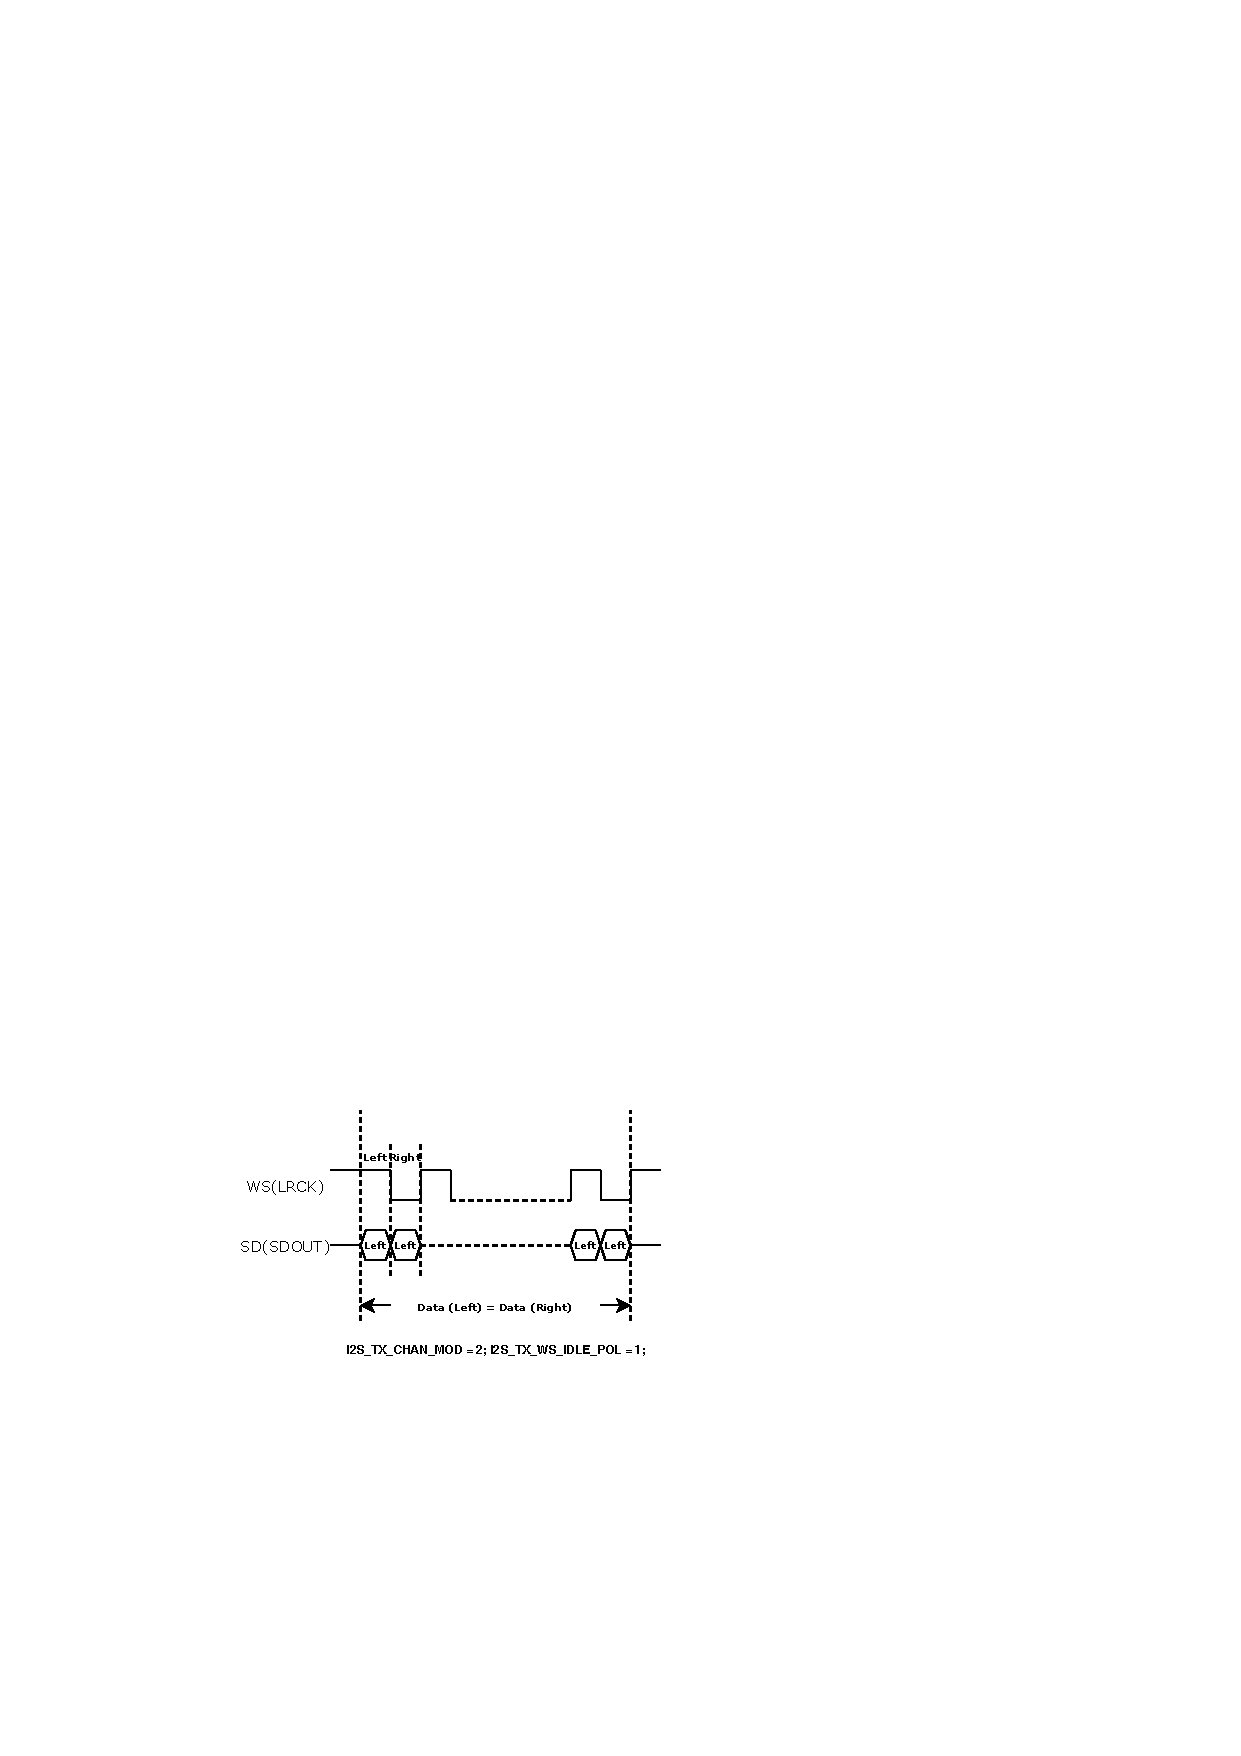
\includegraphics[width=0.8\textwidth]{03-I2S/figures/i2s_chan_mode_20220210.pdf}
    \caption{PDM 通道控制}
    \label{Figure:i2s_channel_mode}
\end{figure}

\section{接收数据}\label{RXCHAN}
\begin{tiplisting}
本小节以及后续小节所述的配置,均需要通过置位 \hyperref[fielddesc:I2SRXUPDATE]{I2S\regindex{n}\_RX\_UPDATE} 的方式来进行更新,从而将 I2S\regindex{n} RX 寄存器数据从 APB 时钟域同步到 I2S\regindex{n} RX 时钟域。详细配置见第 \ref{sec:configure-i2s-as-rx-mode} 小节。
\end{tiplisting}
\vspace{-2em}
I2S\regindex{n} 接收数据时,从外设接口读取数据,经过通道模式控制和数据格式控制,通过 DMA 输入数据至内存。

\subsection{通道模式控制}
\chipname{} I2S\regindex{n} 支持 TDM 和 PDM 两种接收模式。置位 \hyperref[fielddesc:I2SRXTDMEN]{I2S\regindex{n}\_RX\_TDM\_EN} 则为 TDM 接收模式,置位 \hyperref[fielddesc:I2SRXPDMEN]{I2S\regindex{n}\_RX\_PDM\_EN} 则为 PDM 接收模式。

\textbf{注意}:\hyperref[fielddesc:I2SRXTDMEN]{I2S\regindex{n}\_RX\_TDM\_EN} 和 \hyperref[fielddesc:I2SRXPDMEN]{I2S\regindex{n}\_RX\_PDM\_EN} 不能同时置位或同时清零。

\subsubsection{TDM 模式下 I2S\regindex{n} 通道模式}
在 TDM 模式下,I2S\regindex{n} 支持最多 16 通道数据输入。接收通道数由 \hyperref[fielddesc:I2SRXTDMTOTCHANNUM]{I2S\regindex{n}\_RX\_TDM\_TOT\_CHAN\_NUM} 控制。例如,配置 \hyperref[fielddesc:I2SRXTDMTOTCHANNUM]{I2S\regindex{n}\_RX\_TDM\_TOT\_CHAN\_NUM} 为 5,则通道 0 \verb+~+ 5 接收数据。

在接收数据的通道中,如果其对应的 \hyperref[fielddesc:I2STXTDMCHAN0EN]{I2S\regindex{n}\_RX\_TDM\_CHAN{\textcolor{red}{n}}\_EN} 为:
\begin{itemize}
    \item 1,则该通道数据有效,会被存入 RX FIFO。
    \item 0,则该通道数据无效,不会存入 RX FIFO。
\end{itemize}
当 I2S\regindex{n} 处于主机 TDM 模式下,WS 信号由 \hyperref[fielddesc:I2SRXWSIDLEPOL]{I2S\regindex{n}\_RX\_WS\_IDLE\_POL} 和 \hyperref[fielddesc:I2SRXTDMWSWIDTH]{I2S\regindex{n}\_RX\_TDM\_WS\_WIDTH} 控制。其中,\hyperref[fielddesc:I2SRXWSIDLEPOL]{I2S\regindex{n}\_RX\_WS\_IDLE\_POL} 的值为 WS 信号的默认电平,\hyperref[fielddesc:I2SRXTDMWSWIDTH]{I2S\regindex{n}\_RX\_TDM\_WS\_WIDTH} 的值为在接收所有通道的过程中,WS 为默认电平的周期数。另外,\hyperref[fielddesc:I2SRXHALFSAMPLEBITS]{I2S\regindex{n}\_RX\_HALF\_SAMPLE\_BITS} 的值乘以 2,即为一个 WS 周期对应的 BCK 周期数。


\subsubsection{PDM 模式下 I2S\regindex{n} 通道模式}
在 PDM 模式下,I2S\regindex{n} 将通道中的串行数据转换为待输入数据。


当 I2S\regindex{n} 处于主机 PDM 模式下,WS 信号的默认电平由 \hyperref[fielddesc:I2SRXWSIDLEPOL]{I2S\regindex{n}\_RX\_WS\_IDLE\_POL} 控制,WS 信号频率为BCK信号频率的一半,请参考 \ref{The Clock of I2S Module} 小节配置 BCK 信号的方式配置 WS 信号。注意,在 PDM 接收模式下,请配置 \hyperref[fielddesc:I2SRXHALFSAMPLEBITS]{I2S\regindex{n}\_RX\_HALF\_SAMPLE\_BITS} 的值与 \hyperref[fielddesc:I2SRXBITSMOD]{I2S\regindex{n}\_RX\_BITS\_MOD} 的值相同。


I2S\regindex{0} 模块还支持 PDM 转 PCM 输入模式,可以将接收的 PDM 数据转为 PCM 数据,再进行数据控制,配置 \hyperref[fielddesc:I2SRXPDM2PCMEN]{I2S\regindex{0}\_RX\_PDM2PCM\_EN} 启动该模式。PDM 转 PCM 输入模式的寄存器配置如下:
\newline
\begin{itemize}
    \item 配置采样频率和下采样率。\newline
    \chipname{} I2S\regindex{0} PDM 转 PCM 模式下,PDM 时钟频率与主从机模式的关系如下:
    \begin{itemize}
        \item 主机模式:PDM 时钟频率即为 BCK 时钟频率。
        \item 从机模式:PDM 时钟频率由外部提供。
    \end{itemize}
    采样频率 ($f_{\textrm{Sampling}}$) 与 PDM 时钟频率的关系如下:
    $$f_{\textrm{Sampling}} = \frac{f_{\textrm{PDM}}}{\textrm{DSR}}$$
    其中,下采样率 DSR 和 \hyperref[fielddesc:I2SRXPDMSINCDSR16EN]{I2S\regindex{0}\_RX\_PDM\_SINC\_DSR\_16\_EN} 的关系为:
    $${\textrm{DSR}} = {\textrm{\hyperref[fielddesc:I2SRXPDMSINCDSR16EN]{I2S\regindex{0}\_RX\_PDM\_SINC\_DSR\_16\_EN}}} \times {\textrm{64}}$$
    请根据需要的主从机模式、采样频率以及下采样率进行寄存器配置。
    \item 配置有效通道。\newline
    \chipname{} I2S PDM 转 PCM 模式下,最多支持 8 个通道的输入信号,寄存器配置以及对应通道如下表:
\begin{table}[H]
    \centering
    \caption{PDM 转 PCM 输入模式}
    \label{table:PDM_RX_MODE}
    \begin{tabular}{|p{4.3cm}|p{2.0cm}|p{5.8cm}|}
    \hline
    \rowcolor{lightgray}
    \textbf{输入数据信号}&\textbf{通道} &\textbf{使能寄存器} \\ \hline
    \multirow{2}*{I2S\regindex{0}I\_Data\_in}  & 左声道 & \hyperref[fielddesc:I2SRXTDMPDMCHAN0EN]{I2S\regindex{0}\_RX\_TDM\_PDM\_CHAN0\_EN} \\ \cline{2-3}
                                               & 右声道 & \hyperref[fielddesc:I2SRXTDMPDMCHAN0EN]{I2S\regindex{0}\_RX\_TDM\_PDM\_CHAN1\_EN} \\ \hline
    \multirow{2}*{I2S\regindex{0}I1\_Data\_in} & 左声道 & \hyperref[fielddesc:I2SRXTDMPDMCHAN0EN]{I2S\regindex{0}\_RX\_TDM\_PDM\_CHAN2\_EN} \\ \cline{2-3}
                                               & 右声道 & \hyperref[fielddesc:I2SRXTDMPDMCHAN0EN]{I2S\regindex{0}\_RX\_TDM\_PDM\_CHAN3\_EN} \\ \hline
    \multirow{2}*{I2S\regindex{0}I2\_Data\_in} & 左声道 & \hyperref[fielddesc:I2SRXTDMPDMCHAN0EN]{I2S\regindex{0}\_RX\_TDM\_PDM\_CHAN4\_EN} \\ \cline{2-3}
                                               & 右声道 & \hyperref[fielddesc:I2SRXTDMPDMCHAN0EN]{I2S\regindex{0}\_RX\_TDM\_PDM\_CHAN5\_EN} \\ \hline
    \multirow{2}*{I2S\regindex{0}I3\_Data\_in} & 左声道 & \hyperref[fielddesc:I2SRXTDMPDMCHAN0EN]{I2S\regindex{0}\_RX\_TDM\_PDM\_CHAN6\_EN} \\ \cline{2-3}
                                               & 右声道 & \hyperref[fielddesc:I2SRXTDMPDMCHAN0EN]{I2S\regindex{0}\_RX\_TDM\_PDM\_CHAN7\_EN} \\ \hline
    \end{tabular}
\end{table}
\end{itemize}



\subsection{数据格式控制}
数据格式控制分为两个阶段:
\begin{itemize}
    \item 第一阶段从串行数据流输入转换为待输入数据,并存入 RX FIFO;
    \item 第二阶段将待输入数据从 RX FIFO 中读出,并进行输入数据模式转换。
\end{itemize}

\subsubsection{通道数据比特顺序}
\chipname{} I2S\regindex{n} 通道数据比特顺序由 \hyperref[fielddesc:I2SRXBITORDER]{I2S\regindex{n}\_RX\_BIT\_ORDER} 控制,当该值为:
\begin{itemize}
\item 1,串行数据从低位向高位依次存入待输入数据。
\item 0,串行数据从高位向低位依次存入待输入数据。
\end{itemize}
至此,数据格式控制的第一阶段完成。

\subsubsection{通道储存数据位宽}
\hyperref[fielddesc:I2SRXBITSMOD]{I2S\regindex{n}\_RX\_BITS\_MOD} 和 \hyperref[fielddesc:I2SRX24FILLEN]{I2S\regindex{n}\_RX\_24\_FILL\_EN} 决定了每个通道的储存数据位宽,其可取值和对应的储存数据位宽如下表:

\begin{table}[H]
    \centering
    \caption{通道储存数据位宽控制}
    \label{table:RX_BITS_MODE}
    \begin{tabular}{|p{3cm}|R{3.3cm}|R{4cm}|}
    \hline
    \rowcolor{lightgray}
    \textbf{通道储存数据位宽} & \textbf{\hyperref[fielddesc:I2SRXBITSMOD]{I2S\regindex{n}\_RX\_BITS\_MOD}} & \textbf{\hyperref[fielddesc:I2SRX24FILLEN]{I2S\regindex{n}\_RX\_24\_FILL\_EN}}  \\ \hline
    \multirow{2}*{32} & 31 & x \\\cline{2-3}
                 & 23 & 1 \\ \hline
    24 & 23 & 0 \\\hline
    16    & 15 & x \\\hline
    8     & 7 & x \\\hline
    \end{tabular}
\end{table}

\subsubsection{通道接收数据位宽}
\chipname{} I2S\regindex{n} 中,\hyperref[fielddesc:I2SRXTDMCHANBITS]{I2S\regindex{n}\_RX\_TDM\_CHAN\_BITS} 决定了每个通道接收数据的位宽。
\begin{itemize}
\item 当每个通道储存数据位宽小于接收数据的位宽时,接收时仅会在接收数据中取储存位宽作为储存数据。此时,配置 \hyperref[fielddesc:I2SRXLEFTALIGN]{I2S\regindex{n}\_RX\_LEFT\_ALIGN} 为:
\begin{itemize}
\item 0,储存数据位于接收数据低位。
\item 1,储存数据位于接收数据高位。
\end{itemize}
\item 当每个通道接收数据的位宽小于储存数据位宽时,会将接收数据高位补 0,作为储存数据。
\end{itemize}

\subsubsection{通道储存数据字节序}
通道接收数据经过截取/补全后,成为了待储存数据,\hyperref[fielddesc:I2SRXBIGENDIAN]{I2S\regindex{n}\_RX\_BIG\_ENDIAN} 用于控制待储存数据的字节序。下表描述了不同通道储存数据位宽下,该寄存器对待储存数据的控制。
\begin{table}[H]
    \centering
    \caption{通道储存数据字节序控制}
    \label{table:TX_BIG_ENDIAN}
    \begin{tabular}{|p{3cm}|p{3cm}|p{3.5cm}|R{3.5cm}|}
    \hline
    \rowcolor{lightgray}
        \textbf{通道储存数据位宽} & \textbf{原始数据} & \textbf{控制后数据} & \textbf{\hyperref[fielddesc:I2SRXBIGENDIAN]{I2S\regindex{n}\_RX\_BIG\_ENDIAN}} \\ \hline
 \multirow{2}*{32} & \multirow{2}*{\{B3, B2, B1, B0\}} & \{B3, B2, B1, B0\} & 0 \\\cline{3-4}
                      && \{B0, B1, B2, B3\} & 1 \\\hline

    \multirow{2}*{24} & \multirow{2}*{\{B2, B1, B0\}} & \{B2, B1, B0\} & 0 \\\cline{3-4}
                      && \{B0, B1, B2\} & 1 \\\hline

    \multirow{2}*{16} & \multirow{2}*{\{B1, B0\}} & \{B1, B0\} & 0 \\\cline{3-4}
                      && \{B0, B1\} & 1 \\\hline

                8     & \{B0\} & \{B0\} & x \\\hline
    \end{tabular}
\end{table}

\subsubsection{A 率/$\mu$ 率压缩/解压缩}

\chipname{} I2S\regindex{n} 对排列好字节序的待储存数据会按照 32-bit(缺省高位补 0)的方式进行 A 率/$\mu$ 率压缩/解压缩。

配置 \hyperref[fielddesc:I2SRXPCMBYPASS]{I2S\regindex{n}\_RX\_PCM\_BYPASS} 为:
\begin{itemize}
\item 0,则不进行压缩/解压缩
\item 1,则进行压缩/解压缩
\end{itemize}
配置 \hyperref[fielddesc:I2SRXPCMCONF]{I2S\regindex{n}\_RX\_PCM\_CONF} 为:
\begin{itemize}
\item 0,A 律解压缩
\item 1,A 律压缩
\item 2,$\mu$ 律解压缩
\item 3,$\mu$ 律压缩
\end{itemize}
至此,数据格式控制部分全部完成,数据通过 DMA 存入内存。

\section{软件配置流程}
\subsection{软件配置 I2S\regindex{n} 发送流程}\label{sec:configure-i2s-as-tx-mode}
软件配置 I2S\regindex{n} 发送的流程如下:

\begin{enumerate}
    \item 根据 \ref{The Clock of I2S Module} 小节的描述,配置时钟。

    \item 根据表 \ref{table:I2S 信号总线描述} 的描述,配置信号管脚。

    \item 根据主从机模式配置 \hyperref[fielddesc:I2STXSLAVEMOD]{I2S\regindex{n}\_TX\_SLAVE\_MOD}:
    \begin{itemize}
        \item 0:主机发送模式
        \item 1:从机发送模式
    \end{itemize}

    \item 根据 \ref{TXCHAN} 小节的描述,配置正确的发送数据模式和发送通道模式,置位 \hyperref[fielddesc:I2STXUPDATE]{I2S\regindex{n}\_TX\_UPDATE}。

    \item 根据 \ref{i2s_module_reset} 小节的描述,复位发送单元和发送 FIFO。
    \item 根据 \ref{I2S_INT} 小节的描述使能相应的中断。\label{I2S-TX-INTERRUPT}

    \item 配置 DMA 发送链表。

    \item 根据需要置位 \hyperref[fielddesc:I2STXSTOPEN]{I2S\regindex{n}\_TX\_STOP\_EN},更多信息见章节 \ref{subsubsection:master/slave_transmitting_mode}。

    \item 开始发送数据:
    \begin{itemize}
        \item 主机模式下,等待 I2S\regindex{n} 从设备配置完成后,置位 \hyperref[fielddesc:I2STXSTART]{I2S\regindex{n}\_TX\_START} 开始发送数据;
        \item 从机模式下,置位 \hyperref[fielddesc:I2STXSTART]{I2S\regindex{n}\_TX\_START}。I2S\regindex{n} 主设备提供 BCK 和 WS 信号后,开始发送数据。
    \end{itemize}

    \item 等待步骤 \ref{I2S-TX-INTERRUPT} 设置的中断信号,或查询 \hyperref[fielddesc:I2STXIDLE]{I2S\regindex{n}\_TX\_IDLE} 检查传输是否结束:
    \begin{itemize}
        \item 0:发送设备为工作状态;
        \item 1:发送设备为空闲状态。
    \end{itemize}

    \item 清零 \hyperref[fielddesc:I2STXSTART]{I2S\regindex{n}\_TX\_START}。
\end{enumerate}
\subsection{软件配置 I2S\regindex{n} 接收流程}\label{sec:configure-i2s-as-rx-mode}
软件配置 I2S\regindex{n} 接收模式的流程如下:

\begin{enumerate}
    \item 根据 \ref{The Clock of I2S Module} 小节的描述,配置时钟。

    \item 根据表 \ref{table:I2S 信号总线描述} 的描述,配置信号管脚。

    \item 配置 \hyperref[fielddesc:I2SRXSLAVEMOD]{I2S\regindex{n}\_RX\_SLAVE\_MOD} 选择需要的模式:
    \begin{itemize}
        \item 0:主机接收模式
        \item 1:从机接收模式
    \end{itemize}

    \item 根据 \ref{RXCHAN} 小节的描述,配置正确的接收通道模式和接收数据模式,置位 \hyperref[fielddesc:I2SRXUPDATE]{I2S\regindex{n}\_RX\_UPDATE}。

    \item 根据 \ref{i2s_module_reset} 小节的描述,复位接收单元和接收 FIFO。
    \item 根据 \ref{I2S_INT} 小节的描述使能相应的中断。\label{I2S-RX-INTERRUPT}

    \item 配置 DMA 接收链表,并在 \hyperref[regdesc:I2SRXEOFNUMREG]{I2S\regindex{n}\_RXEOF\_NUM\_REG} 中配置接收数据长度。

    \item 开始接收数据:
    \begin{itemize}
        \item 在主机模式下,等待从机准备好后,置位 \hyperref[fielddesc:I2SRXSTART]{I2S\regindex{n}\_RX\_START} 开始接收数据;
        \item 在从机模式下,置位 \hyperref[fielddesc:I2SRXSTART]{I2S\regindex{n}\_RX\_START},等待主机提供 BCK 和 WS 信号后开始接收数据。
    \end{itemize}
    \item 接收的数据由 DMA 根据配置,存到 \chipname{} 存储器的指定地址。最终产生步骤 \ref{I2S-RX-INTERRUPT} 中设置的中断。
\end{enumerate}


\section{I2S\regindex{n} 中断} \label{I2S_INT}
%\subsection{FIFO 中断}

\begin{itemize}
\item \label{int:I2STXHUNGINT}I2S\_TX\_HUNG\_INT:当发送数据超时即触发此中断。例如,I2S\regindex{n} 配置为从机发送模式,但主机长时间未提供 BCK 或 WS 信号,则将触发该中断。超时配置见寄存器 \hyperref[regdesc:I2SLCHUNGCONFREG]{I2S\regindex{n}\_LC\_HUNG\_CONF\_REG}。
\item \label{int:I2SRXHUNGINT}I2S\_RX\_HUNG\_INT:当接收数据超时即触发此中断。例如,I2S\regindex{n} 配置为从机接收模式,但主机长时间未发送数据,则将触发该中断。超时配置见寄存器 \hyperref[regdesc:I2SLCHUNGCONFREG]{I2S\regindex{n}\_LC\_HUNG\_CONF\_REG}。
\item \label{int:I2STXDONEINT}I2S\_TX\_DONE\_INT:当发送数据完成即触发此中断。
\item \label{int:I2SRXDONEINT}I2S\_RX\_DONE\_INT:当接收数据完成即触发此中断。
\end{itemize}

\hypertarget{i2s-reg-summ}{}
\section{寄存器列表}


本小节的所有地址均为相对于 [I2S\regindex{n}] 的地址偏移量(相对地址),具体基地址请见章节 \ref{mod:sysmem} \textit{\nameref{mod:sysmem}} 中的表 \ref{tab:sysmem-base-address}。
%\subsection{I2S0 寄存器列表}

请查看章节 \hyperref[glossary-access-types]{\textit{寄存器的访问类型}},了解“访问”列缩写的含义。

\subfile{03-I2S/03-I2S-reg-summ__CN}

%\subsection{I2S1 寄存器列表}

%\subfile{03-I2S/i2s1_reg_summary.tex}

\section{寄存器}\label{I2SRegister}

%\subsection{I2S0 寄存器}
\subfile{03-I2S/03-I2S-reg__CN}

%\subsection{I2S1 寄存器}
%\subfile{03-I2S/i2s1_reg.tex}
\end{document}